\documentclass{article} % For LaTeX2e
\usepackage[T1]{fontenc}
\usepackage{iclr2025_conference,times}
\iclrfinalcopy % not anonymous: an internal report, not a double-blind submission

% Optional math commands from https://github.com/goodfeli/dlbook_notation.
%%%%% NEW MATH DEFINITIONS %%%%%

\usepackage{amsmath,amsfonts,bm}

% Mark sections of captions for referring to divisions of figures
\newcommand{\figleft}{{\em (Left)}}
\newcommand{\figcenter}{{\em (Center)}}
\newcommand{\figright}{{\em (Right)}}
\newcommand{\figtop}{{\em (Top)}}
\newcommand{\figbottom}{{\em (Bottom)}}
\newcommand{\captiona}{{\em (a)}}
\newcommand{\captionb}{{\em (b)}}
\newcommand{\captionc}{{\em (c)}}
\newcommand{\captiond}{{\em (d)}}

% Highlight a newly defined term
\newcommand{\newterm}[1]{{\bf #1}}


% Figure reference, lower-case.
\def\figref#1{figure~\ref{#1}}
% Figure reference, capital. For start of sentence
\def\Figref#1{Figure~\ref{#1}}
\def\twofigref#1#2{figures \ref{#1} and \ref{#2}}
\def\quadfigref#1#2#3#4{figures \ref{#1}, \ref{#2}, \ref{#3} and \ref{#4}}
% Section reference, lower-case.
\def\secref#1{section~\ref{#1}}
% Section reference, capital.
\def\Secref#1{Section~\ref{#1}}
% Reference to two sections.
\def\twosecrefs#1#2{sections \ref{#1} and \ref{#2}}
% Reference to three sections.
\def\secrefs#1#2#3{sections \ref{#1}, \ref{#2} and \ref{#3}}
% Reference to an equation, lower-case.
\def\eqref#1{equation~\ref{#1}}
% Reference to an equation, upper case
\def\Eqref#1{Equation~\ref{#1}}
% A raw reference to an equation---avoid using if possible
\def\plaineqref#1{\ref{#1}}
% Reference to a chapter, lower-case.
\def\chapref#1{chapter~\ref{#1}}
% Reference to an equation, upper case.
\def\Chapref#1{Chapter~\ref{#1}}
% Reference to a range of chapters
\def\rangechapref#1#2{chapters\ref{#1}--\ref{#2}}
% Reference to an algorithm, lower-case.
\def\algref#1{algorithm~\ref{#1}}
% Reference to an algorithm, upper case.
\def\Algref#1{Algorithm~\ref{#1}}
\def\twoalgref#1#2{algorithms \ref{#1} and \ref{#2}}
\def\Twoalgref#1#2{Algorithms \ref{#1} and \ref{#2}}
% Reference to a part, lower case
\def\partref#1{part~\ref{#1}}
% Reference to a part, upper case
\def\Partref#1{Part~\ref{#1}}
\def\twopartref#1#2{parts \ref{#1} and \ref{#2}}

\def\ceil#1{\lceil #1 \rceil}
\def\floor#1{\lfloor #1 \rfloor}
\def\1{\bm{1}}
\newcommand{\train}{\mathcal{D}}
\newcommand{\valid}{\mathcal{D_{\mathrm{valid}}}}
\newcommand{\test}{\mathcal{D_{\mathrm{test}}}}

\def\eps{{\epsilon}}


% Random variables
\def\reta{{\textnormal{$\eta$}}}
\def\ra{{\textnormal{a}}}
\def\rb{{\textnormal{b}}}
\def\rc{{\textnormal{c}}}
\def\rd{{\textnormal{d}}}
\def\re{{\textnormal{e}}}
\def\rf{{\textnormal{f}}}
\def\rg{{\textnormal{g}}}
\def\rh{{\textnormal{h}}}
\def\ri{{\textnormal{i}}}
\def\rj{{\textnormal{j}}}
\def\rk{{\textnormal{k}}}
\def\rl{{\textnormal{l}}}
% rm is already a command, just don't name any random variables m
\def\rn{{\textnormal{n}}}
\def\ro{{\textnormal{o}}}
\def\rp{{\textnormal{p}}}
\def\rq{{\textnormal{q}}}
\def\rr{{\textnormal{r}}}
\def\rs{{\textnormal{s}}}
\def\rt{{\textnormal{t}}}
\def\ru{{\textnormal{u}}}
\def\rv{{\textnormal{v}}}
\def\rw{{\textnormal{w}}}
\def\rx{{\textnormal{x}}}
\def\ry{{\textnormal{y}}}
\def\rz{{\textnormal{z}}}

% Random vectors
\def\rvepsilon{{\mathbf{\epsilon}}}
\def\rvtheta{{\mathbf{\theta}}}
\def\rva{{\mathbf{a}}}
\def\rvb{{\mathbf{b}}}
\def\rvc{{\mathbf{c}}}
\def\rvd{{\mathbf{d}}}
\def\rve{{\mathbf{e}}}
\def\rvf{{\mathbf{f}}}
\def\rvg{{\mathbf{g}}}
\def\rvh{{\mathbf{h}}}
\def\rvu{{\mathbf{i}}}
\def\rvj{{\mathbf{j}}}
\def\rvk{{\mathbf{k}}}
\def\rvl{{\mathbf{l}}}
\def\rvm{{\mathbf{m}}}
\def\rvn{{\mathbf{n}}}
\def\rvo{{\mathbf{o}}}
\def\rvp{{\mathbf{p}}}
\def\rvq{{\mathbf{q}}}
\def\rvr{{\mathbf{r}}}
\def\rvs{{\mathbf{s}}}
\def\rvt{{\mathbf{t}}}
\def\rvu{{\mathbf{u}}}
\def\rvv{{\mathbf{v}}}
\def\rvw{{\mathbf{w}}}
\def\rvx{{\mathbf{x}}}
\def\rvy{{\mathbf{y}}}
\def\rvz{{\mathbf{z}}}

% Elements of random vectors
\def\erva{{\textnormal{a}}}
\def\ervb{{\textnormal{b}}}
\def\ervc{{\textnormal{c}}}
\def\ervd{{\textnormal{d}}}
\def\erve{{\textnormal{e}}}
\def\ervf{{\textnormal{f}}}
\def\ervg{{\textnormal{g}}}
\def\ervh{{\textnormal{h}}}
\def\ervi{{\textnormal{i}}}
\def\ervj{{\textnormal{j}}}
\def\ervk{{\textnormal{k}}}
\def\ervl{{\textnormal{l}}}
\def\ervm{{\textnormal{m}}}
\def\ervn{{\textnormal{n}}}
\def\ervo{{\textnormal{o}}}
\def\ervp{{\textnormal{p}}}
\def\ervq{{\textnormal{q}}}
\def\ervr{{\textnormal{r}}}
\def\ervs{{\textnormal{s}}}
\def\ervt{{\textnormal{t}}}
\def\ervu{{\textnormal{u}}}
\def\ervv{{\textnormal{v}}}
\def\ervw{{\textnormal{w}}}
\def\ervx{{\textnormal{x}}}
\def\ervy{{\textnormal{y}}}
\def\ervz{{\textnormal{z}}}

% Random matrices
\def\rmA{{\mathbf{A}}}
\def\rmB{{\mathbf{B}}}
\def\rmC{{\mathbf{C}}}
\def\rmD{{\mathbf{D}}}
\def\rmE{{\mathbf{E}}}
\def\rmF{{\mathbf{F}}}
\def\rmG{{\mathbf{G}}}
\def\rmH{{\mathbf{H}}}
\def\rmI{{\mathbf{I}}}
\def\rmJ{{\mathbf{J}}}
\def\rmK{{\mathbf{K}}}
\def\rmL{{\mathbf{L}}}
\def\rmM{{\mathbf{M}}}
\def\rmN{{\mathbf{N}}}
\def\rmO{{\mathbf{O}}}
\def\rmP{{\mathbf{P}}}
\def\rmQ{{\mathbf{Q}}}
\def\rmR{{\mathbf{R}}}
\def\rmS{{\mathbf{S}}}
\def\rmT{{\mathbf{T}}}
\def\rmU{{\mathbf{U}}}
\def\rmV{{\mathbf{V}}}
\def\rmW{{\mathbf{W}}}
\def\rmX{{\mathbf{X}}}
\def\rmY{{\mathbf{Y}}}
\def\rmZ{{\mathbf{Z}}}

% Elements of random matrices
\def\ermA{{\textnormal{A}}}
\def\ermB{{\textnormal{B}}}
\def\ermC{{\textnormal{C}}}
\def\ermD{{\textnormal{D}}}
\def\ermE{{\textnormal{E}}}
\def\ermF{{\textnormal{F}}}
\def\ermG{{\textnormal{G}}}
\def\ermH{{\textnormal{H}}}
\def\ermI{{\textnormal{I}}}
\def\ermJ{{\textnormal{J}}}
\def\ermK{{\textnormal{K}}}
\def\ermL{{\textnormal{L}}}
\def\ermM{{\textnormal{M}}}
\def\ermN{{\textnormal{N}}}
\def\ermO{{\textnormal{O}}}
\def\ermP{{\textnormal{P}}}
\def\ermQ{{\textnormal{Q}}}
\def\ermR{{\textnormal{R}}}
\def\ermS{{\textnormal{S}}}
\def\ermT{{\textnormal{T}}}
\def\ermU{{\textnormal{U}}}
\def\ermV{{\textnormal{V}}}
\def\ermW{{\textnormal{W}}}
\def\ermX{{\textnormal{X}}}
\def\ermY{{\textnormal{Y}}}
\def\ermZ{{\textnormal{Z}}}

% Vectors
\def\vzero{{\bm{0}}}
\def\vone{{\bm{1}}}
\def\vmu{{\bm{\mu}}}
\def\vtheta{{\bm{\theta}}}
\def\va{{\bm{a}}}
\def\vb{{\bm{b}}}
\def\vc{{\bm{c}}}
\def\vd{{\bm{d}}}
\def\ve{{\bm{e}}}
\def\vf{{\bm{f}}}
\def\vg{{\bm{g}}}
\def\vh{{\bm{h}}}
\def\vi{{\bm{i}}}
\def\vj{{\bm{j}}}
\def\vk{{\bm{k}}}
\def\vl{{\bm{l}}}
\def\vm{{\bm{m}}}
\def\vn{{\bm{n}}}
\def\vo{{\bm{o}}}
\def\vp{{\bm{p}}}
\def\vq{{\bm{q}}}
\def\vr{{\bm{r}}}
\def\vs{{\bm{s}}}
\def\vt{{\bm{t}}}
\def\vu{{\bm{u}}}
\def\vv{{\bm{v}}}
\def\vw{{\bm{w}}}
\def\vx{{\bm{x}}}
\def\vy{{\bm{y}}}
\def\vz{{\bm{z}}}

% Elements of vectors
\def\evalpha{{\alpha}}
\def\evbeta{{\beta}}
\def\evepsilon{{\epsilon}}
\def\evlambda{{\lambda}}
\def\evomega{{\omega}}
\def\evmu{{\mu}}
\def\evpsi{{\psi}}
\def\evsigma{{\sigma}}
\def\evtheta{{\theta}}
\def\eva{{a}}
\def\evb{{b}}
\def\evc{{c}}
\def\evd{{d}}
\def\eve{{e}}
\def\evf{{f}}
\def\evg{{g}}
\def\evh{{h}}
\def\evi{{i}}
\def\evj{{j}}
\def\evk{{k}}
\def\evl{{l}}
\def\evm{{m}}
\def\evn{{n}}
\def\evo{{o}}
\def\evp{{p}}
\def\evq{{q}}
\def\evr{{r}}
\def\evs{{s}}
\def\evt{{t}}
\def\evu{{u}}
\def\evv{{v}}
\def\evw{{w}}
\def\evx{{x}}
\def\evy{{y}}
\def\evz{{z}}

% Matrix
\def\mA{{\bm{A}}}
\def\mB{{\bm{B}}}
\def\mC{{\bm{C}}}
\def\mD{{\bm{D}}}
\def\mE{{\bm{E}}}
\def\mF{{\bm{F}}}
\def\mG{{\bm{G}}}
\def\mH{{\bm{H}}}
\def\mI{{\bm{I}}}
\def\mJ{{\bm{J}}}
\def\mK{{\bm{K}}}
\def\mL{{\bm{L}}}
\def\mM{{\bm{M}}}
\def\mN{{\bm{N}}}
\def\mO{{\bm{O}}}
\def\mP{{\bm{P}}}
\def\mQ{{\bm{Q}}}
\def\mR{{\bm{R}}}
\def\mS{{\bm{S}}}
\def\mT{{\bm{T}}}
\def\mU{{\bm{U}}}
\def\mV{{\bm{V}}}
\def\mW{{\bm{W}}}
\def\mX{{\bm{X}}}
\def\mY{{\bm{Y}}}
\def\mZ{{\bm{Z}}}
\def\mBeta{{\bm{\beta}}}
\def\mPhi{{\bm{\Phi}}}
\def\mLambda{{\bm{\Lambda}}}
\def\mSigma{{\bm{\Sigma}}}

% Tensor
\DeclareMathAlphabet{\mathsfit}{\encodingdefault}{\sfdefault}{m}{sl}
\SetMathAlphabet{\mathsfit}{bold}{\encodingdefault}{\sfdefault}{bx}{n}
\newcommand{\tens}[1]{\bm{\mathsfit{#1}}}
\def\tA{{\tens{A}}}
\def\tB{{\tens{B}}}
\def\tC{{\tens{C}}}
\def\tD{{\tens{D}}}
\def\tE{{\tens{E}}}
\def\tF{{\tens{F}}}
\def\tG{{\tens{G}}}
\def\tH{{\tens{H}}}
\def\tI{{\tens{I}}}
\def\tJ{{\tens{J}}}
\def\tK{{\tens{K}}}
\def\tL{{\tens{L}}}
\def\tM{{\tens{M}}}
\def\tN{{\tens{N}}}
\def\tO{{\tens{O}}}
\def\tP{{\tens{P}}}
\def\tQ{{\tens{Q}}}
\def\tR{{\tens{R}}}
\def\tS{{\tens{S}}}
\def\tT{{\tens{T}}}
\def\tU{{\tens{U}}}
\def\tV{{\tens{V}}}
\def\tW{{\tens{W}}}
\def\tX{{\tens{X}}}
\def\tY{{\tens{Y}}}
\def\tZ{{\tens{Z}}}


% Graph
\def\gA{{\mathcal{A}}}
\def\gB{{\mathcal{B}}}
\def\gC{{\mathcal{C}}}
\def\gD{{\mathcal{D}}}
\def\gE{{\mathcal{E}}}
\def\gF{{\mathcal{F}}}
\def\gG{{\mathcal{G}}}
\def\gH{{\mathcal{H}}}
\def\gI{{\mathcal{I}}}
\def\gJ{{\mathcal{J}}}
\def\gK{{\mathcal{K}}}
\def\gL{{\mathcal{L}}}
\def\gM{{\mathcal{M}}}
\def\gN{{\mathcal{N}}}
\def\gO{{\mathcal{O}}}
\def\gP{{\mathcal{P}}}
\def\gQ{{\mathcal{Q}}}
\def\gR{{\mathcal{R}}}
\def\gS{{\mathcal{S}}}
\def\gT{{\mathcal{T}}}
\def\gU{{\mathcal{U}}}
\def\gV{{\mathcal{V}}}
\def\gW{{\mathcal{W}}}
\def\gX{{\mathcal{X}}}
\def\gY{{\mathcal{Y}}}
\def\gZ{{\mathcal{Z}}}

% Sets
\def\sA{{\mathbb{A}}}
\def\sB{{\mathbb{B}}}
\def\sC{{\mathbb{C}}}
\def\sD{{\mathbb{D}}}
% Don't use a set called E, because this would be the same as our symbol
% for expectation.
\def\sF{{\mathbb{F}}}
\def\sG{{\mathbb{G}}}
\def\sH{{\mathbb{H}}}
\def\sI{{\mathbb{I}}}
\def\sJ{{\mathbb{J}}}
\def\sK{{\mathbb{K}}}
\def\sL{{\mathbb{L}}}
\def\sM{{\mathbb{M}}}
\def\sN{{\mathbb{N}}}
\def\sO{{\mathbb{O}}}
\def\sP{{\mathbb{P}}}
\def\sQ{{\mathbb{Q}}}
\def\sR{{\mathbb{R}}}
\def\sS{{\mathbb{S}}}
\def\sT{{\mathbb{T}}}
\def\sU{{\mathbb{U}}}
\def\sV{{\mathbb{V}}}
\def\sW{{\mathbb{W}}}
\def\sX{{\mathbb{X}}}
\def\sY{{\mathbb{Y}}}
\def\sZ{{\mathbb{Z}}}

% Entries of a matrix
\def\emLambda{{\Lambda}}
\def\emA{{A}}
\def\emB{{B}}
\def\emC{{C}}
\def\emD{{D}}
\def\emE{{E}}
\def\emF{{F}}
\def\emG{{G}}
\def\emH{{H}}
\def\emI{{I}}
\def\emJ{{J}}
\def\emK{{K}}
\def\emL{{L}}
\def\emM{{M}}
\def\emN{{N}}
\def\emO{{O}}
\def\emP{{P}}
\def\emQ{{Q}}
\def\emR{{R}}
\def\emS{{S}}
\def\emT{{T}}
\def\emU{{U}}
\def\emV{{V}}
\def\emW{{W}}
\def\emX{{X}}
\def\emY{{Y}}
\def\emZ{{Z}}
\def\emSigma{{\Sigma}}

% entries of a tensor
% Same font as tensor, without \bm wrapper
\newcommand{\etens}[1]{\mathsfit{#1}}
\def\etLambda{{\etens{\Lambda}}}
\def\etA{{\etens{A}}}
\def\etB{{\etens{B}}}
\def\etC{{\etens{C}}}
\def\etD{{\etens{D}}}
\def\etE{{\etens{E}}}
\def\etF{{\etens{F}}}
\def\etG{{\etens{G}}}
\def\etH{{\etens{H}}}
\def\etI{{\etens{I}}}
\def\etJ{{\etens{J}}}
\def\etK{{\etens{K}}}
\def\etL{{\etens{L}}}
\def\etM{{\etens{M}}}
\def\etN{{\etens{N}}}
\def\etO{{\etens{O}}}
\def\etP{{\etens{P}}}
\def\etQ{{\etens{Q}}}
\def\etR{{\etens{R}}}
\def\etS{{\etens{S}}}
\def\etT{{\etens{T}}}
\def\etU{{\etens{U}}}
\def\etV{{\etens{V}}}
\def\etW{{\etens{W}}}
\def\etX{{\etens{X}}}
\def\etY{{\etens{Y}}}
\def\etZ{{\etens{Z}}}

% The true underlying data generating distribution
\newcommand{\pdata}{p_{\rm{data}}}
% The empirical distribution defined by the training set
\newcommand{\ptrain}{\hat{p}_{\rm{data}}}
\newcommand{\Ptrain}{\hat{P}_{\rm{data}}}
% The model distribution
\newcommand{\pmodel}{p_{\rm{model}}}
\newcommand{\Pmodel}{P_{\rm{model}}}
\newcommand{\ptildemodel}{\tilde{p}_{\rm{model}}}
% Stochastic autoencoder distributions
\newcommand{\pencode}{p_{\rm{encoder}}}
\newcommand{\pdecode}{p_{\rm{decoder}}}
\newcommand{\precons}{p_{\rm{reconstruct}}}

\newcommand{\laplace}{\mathrm{Laplace}} % Laplace distribution

\newcommand{\E}{\mathbb{E}}
\newcommand{\Ls}{\mathcal{L}}
\newcommand{\R}{\mathbb{R}}
\newcommand{\emp}{\tilde{p}}
\newcommand{\lr}{\alpha}
\newcommand{\reg}{\lambda}
\newcommand{\rect}{\mathrm{rectifier}}
\newcommand{\softmax}{\mathrm{softmax}}
\newcommand{\sigmoid}{\sigma}
\newcommand{\softplus}{\zeta}
\newcommand{\KL}{D_{\mathrm{KL}}}
\newcommand{\Var}{\mathrm{Var}}
\newcommand{\standarderror}{\mathrm{SE}}
\newcommand{\Cov}{\mathrm{Cov}}
% Wolfram Mathworld says $L^2$ is for function spaces and $\ell^2$ is for vectors
% But then they seem to use $L^2$ for vectors throughout the site, and so does
% wikipedia.
\newcommand{\normlzero}{L^0}
\newcommand{\normlone}{L^1}
\newcommand{\normltwo}{L^2}
\newcommand{\normlp}{L^p}
\newcommand{\normmax}{L^\infty}

\newcommand{\parents}{Pa} % See usage in notation.tex. Chosen to match Daphne's book.

\DeclareMathOperator*{\argmax}{arg\,max}
\DeclareMathOperator*{\argmin}{arg\,min}

\DeclareMathOperator{\sign}{sign}
\DeclareMathOperator{\Tr}{Tr}
\let\ab\allowbreak


\usepackage{hyperref}
\usepackage{url}
\usepackage{booktabs}
\usepackage{graphicx}

% Human results not yet in print as a boxed "pending" marker; see human_results.tex
% Values of the human results (calibration, audit, triage, adjudication, bias sheets).
% \HR{<id>} prints the value when it is defined here, and a boxed "pending" marker until then.
% The ids are listed in reports/paper_v4/materials/pending_human_results.md.
% Do not edit by hand: analysis/paper_v4/fill_human_results.py writes the definitions below.
\makeatletter
\newcommand{\HR}[1]{\@ifundefined{hr@#1}{\fbox{\scriptsize\textsf{pending:\,\detokenize{#1}}}}{\@nameuse{hr@#1}}}
\makeatother
% ---- values (none yet, 2026-11-20) ----


%%%%%%%%% TITLE - PLEASE UPDATE TITLE HERE
\title{GP-RareLink: Provenance-First Genotype--Phenotype Records from Rare-Disease Case Reports, Scored Against Held-Out Databases (Interim Report, Version~4)}

\author{Jimmy Lin \\
Rare Genomics Institute
\And
Monica S. Lam \\
Stanford University, Open Virtual Assistant Lab
}

\newcommand{\fix}{\marginpar{FIX}}
\newcommand{\new}{\marginpar{NEW}}

\begin{document}

\maketitle

\begin{abstract}
%%%%%%%%% ABSTRACT %%%%%%%%%
Rare-disease variants described in case reports often never reach ClinVar or OMIM. GP-RareLink asks whether an LLM-based systematic-review method (SLIDERS), run with Claude, can turn case reports into variant--phenotype--disease records that a person can check value by value, at a demonstrable accuracy. This interim report establishes provenance and feasibility; it does not yet establish accuracy. Claude Opus writes per-person records in which every value carries the PMID and a verbatim quote and phenotypes are three-state; a second Claude read (the gatekeeper) removes claims their quote does not support; ClinVar and OMIM are held out of extraction and used only to score it; plan and pipeline were frozen on 2026-10-20. The only human audits so far, two single-rater pilot audits on the development disease before the freeze, found 6.0\% (3/50) and 6.3\% (3/48) of claims unsupported, above the 2\% target, and the gatekeeper flagged only 2 of 6 and 1 of 4 of the claims the rater rejected. In six registered diseases, 350 papers gave 2,836 schema-valid GA4GH Phenopackets; all 241,730 asserted values carry a verbatim quote, which holds by construction and was confirmed by a span check. The gatekeeper judged 0.43\% (248/57,819) of claims unsupported in the five confirmatory diseases: a screen of measured low sensitivity, not an error rate. HGVS recall against ClinVar is 10.1\%--35.0\% at tier~1, causes untriaged; 57.3\% (43/75) of OMIM's allelic variants are recovered; 214 gap candidates in the registered six (269 across all twelve diseases studied) await adjudication, and none is yet shown to be a real gap. The pending 250-claim human audit (\HR{o1_unsupported_n} of 250 unsupported; \HR{o1_unsupported_pct}; exact 95\% CI \HR{o1_unsupported_ci}) will decide whether the registered pipeline meets the 2\% target; triage and adjudication will decide what the misses and candidates mean.
%%%%%%%%% ABSTRACT %%%%%%%%%
\end{abstract}

\section{Introduction}
\label{sec:intro}
%%%%%%%%% INTRODUCTION %%%%%%%%%
Rare diseases together affect an estimated 3.5--5.9\% of the population \citep{Wakap2019EstimatingCumulative} and diagnosis in Europe takes close to five years on average \citep{Faye2024TimeDiagnosis}; a diagnosis often depends on finding evidence that already exists. That evidence is fragmented across ClinVar \citep{landrum2025_clinvar}, OMIM \citep{amberger2019_omim}, the Human Phenotype Ontology (HPO) \citep{gargano2024_hpo}, Mondo \citep{vasilevsky2025_mondo} and Monarch's phenopacket-store \citep{danis2025_phenopacket_store}, while most individual patients are described only in case reports. A laboratory querying ClinVar cannot see a causative variant that was published but never submitted: in one curated gene, 24\% of the pathogenic variants found in PubMed articles were absent from every database examined \citep{Lyons2023RareDisease}, and a full-text study reports more than 60,000 likely disease-causing HGMD variants absent from ClinVar \citep{birgmeier2020_avada}. Non-standard variant names hide evidence \citep{freeman2024_vv_literature,lansdon2026_nomenclature_errors}, and phenotype detail in first reports is often superficial \citep{almail2024_reporting_gaps}.

Alexander disease shows the size of the gap: a 2024 systematic review reports 550 patients and 182 causative \emph{GFAP} variants \citep{grossi2024_axd_meta}, against 76 pathogenic or likely pathogenic (P/LP) single-gene \emph{GFAP} records in ClinVar's release of 2026-10-12 and 13 allelic variants in OMIM's gene entry (frozen 2026-10-28). None of the twelve genes studied here has a phenopacket-store folder (commit \texttt{ca133e6}, 2026-11-04). LLM evaluation in rare disease has mostly targeted diagnosis, where LLMs trail a traditional decision-support tool on phenopacket-derived cases \citep{reese2026_llm_vs_exomiser} and leakage puts most studies at high risk of bias \citep{nguyen2026_llm_rd_metaanalysis}; building case-level records with an error rate measured by people has received less attention.

GP-RareLink asks whether SLIDERS \citep{joshi2026_sliders}, a systematic-review method that builds evidence tables with verbatim excerpts as provenance and reconciles them with a code-writing agent, can, run with Claude, build such records at an accuracy we can demonstrate. Every extracted value carries a verbatim quote and the PMID; phenotypes are three-state and ``not reported'' is never collapsed into ``excluded''; a second Claude read, the \emph{gatekeeper}, removes values their quote does not support; the output is GA4GH Phenopackets v2. ClinVar and OMIM are never read by extraction, so that afterwards they can score it (O2) and expose variants absent from both (gap candidates, O3). People decide what counts: an audit of values against their quotes (O1, primary: fewer than 2\% unsupported in 250 claims), a triage of ClinVar misses and adjudication of gap candidates; nothing goes to a database without the panel's approval and the PI's sign-off. The \emph{registered study} is six diseases (Table~\ref{tab:diseases}); its pooled headline figures exclude HA20, the development disease. Five reserve diseases run under a separately pre-registered extension, one exploratory disease and a corpus addendum of free copies found after the freeze are reported apart and never pooled with it (Section~\ref{sec:beside}).

\paragraph{What this report can and cannot claim.} This is version~4 of an internal interim report, written before any person has rated output of the frozen pipeline; every human result is a boxed placeholder that a script fills (Table~\ref{tab:status}). It is a report on provenance and feasibility. The only accuracy evidence from people is two pre-freeze single-rater pilot audits, both above target (Section~\ref{sec:accuracy}). We contribute (i) a provenance-first pipeline from case reports to validated phenopackets, run frozen on the registered six (350 papers, 2,836 phenopackets) and, apart, on six more diseases; (ii) a database-held-out evaluation whose human parts (audit sample, triage sample, 214 gap candidates in the registered six with evidence dossiers) are drawn and waiting for people; and (iii) an account of what is not yet known, stated so that the pending results can settle it.

\begin{table}[t]
\caption{Status at a glance, registered six unless stated (2026-11-20). ``Done'' gives what is measured, with denominators; ``pending'' cells print a marker until people's ratings fill them. Gatekeeper figures are model readings, not error rates.}
\label{tab:status}
\begin{center}
\scriptsize
\setlength{\tabcolsep}{3pt}
\begin{tabular}{p{1.9cm}p{5.9cm}p{5.4cm}}
\toprule
Outcome & Done (measured) & Pending (what people will decide) \\
\midrule
Provenance & 241,730 values, all with a verbatim quote; 0 span-check problems (an unquoted value is not emitted) & -- \\
O1 accuracy (primary) & 250 claims drawn (seed 40250) before any concordance; pilot audits 6.0\% (3/50), 6.3\% (3/48), pre-freeze & \HR{o1_unsupported_n} of 250; rule C \HR{o1_rule_c} \\
Gatekeeper screen & removed as unsupported 0.43\% (248/57,819, five confirmatory); pilot detection 2 of 6 and 1 of 4 & caught on O1: \HR{o1_gatekeeper_sens} \\
O2 ClinVar & tier-1 HGVS recall 10.1\%--35.0\%; tier-1 overlap 35\%--87\% (not precision) & 50 misses: \HR{o2_triage_breakdown} \\
OMIM holdout & 57.3\% (43/75) allelic variants recovered; phenotype half not assessed & -- \\
O3 gap candidates & 214 left for the panel, all with dossiers (269 in all twelve) & accepted \HR{o3_accepted} \\
O4 bias & memorization probe on 180 papers; primary denominators fixed; no sheet filled & \HR{o4_deviation} \\
O5 efficiency & open-weight run screened by the gatekeeper; pilot 0.37--0.65 min per rating & \HR{o5_minutes_per_record}; \HR{o5_openweight_audit} \\
Calibration & 40 claims (20/20) and floor fixed; 9 raters invited, due 2026-11-22 & at floor: \HR{cal_raters_pass} \\
\bottomrule
\end{tabular}
\end{center}
\end{table}
%%%%%%%%% INTRODUCTION %%%%%%%%%

\section{Related Work}
\label{sec:related_work}
%%%%%%%%% RELATED WORK %%%%%%%%%
\paragraph{Variant and phenotype extraction.} tmVar~3.0 normalizes variant mentions \citep{wei2022_tmvar3} and LitVar~2.0 indexes about 15 million variants against papers \citep{allot2023_litvar2}; its ClinVar links are kept out of our extraction. AVADA recovered 59\% of HGMD's disease-causing variants from full text \citep{birgmeier2020_avada}; PubMind finds about 10\% of its mapped variants in ClinVar \citep{wang2025_pubmind}; and when GPT-4o, Claude Opus~4 and DeepSeek-V3 extracted disease genes from full text, disease and phenotype fields were error-prone for all three \citep{yin2025_llm_disease_genes}. One result bears on our proband counting and is unfavorable for Claude: among five models counting probands for PS4, Claude Sonnet~4 had the lowest exact-count concordance (73.0\%, against 91.1\% for the best) and the lowest stability \citep{murugan2026_reasoning_llm_ps4}. For HPO, RAG-HPO reached a best F1 of 0.78 on 112 case reports \citep{garcia2025_raghpo}; GPT recognition was non-deterministic \citep{groza2024_gpt_hpo}. The 97.6\% HPO precision for Claude Sonnet~4.5 quoted in the project's application \citep{larsen2026_hpo_mcp} comes from four synthetic clinical notes in a tool-augmented condition (80.7\% without tools), with recall 65.3\%, and Claude was not top on precision or F1. GP-RareLink is compared with no tagger; its contribution is the quoted, three-state per-person record and its held-out evaluation.

\paragraph{Evidence synthesis and claim verification.} LLM extraction for evidence synthesis has been reviewed systematically \citep{Shankar2026PerformanceLarge}: numeric fields fare worse than text \citep{kataoka2025_gpt4o_o3_extraction}, reproducibility fell from 94.1\% to 77.2\% when information was not reported \citep{Jensen2025Chatgpt4oCan}, and otto-SR reached 93.1\% extraction accuracy against 79.7\% for humans \citep{cao2025_ottosr}. SLIDERS comes from the Lam lab, whose WikiChat grounds and verifies claims \citep{semnani2023_wikichat}. AIS defines support by a cited span \citep{rashkin2023_ais}, the gatekeeper's criterion; FActScore checks atomic claims \citep{min2023_factscore}, our audit unit; self-verification of cited spans improved clinical extraction \citep{gero2023_self_verification}; and clinical fact-checkers have been validated against clinician labels \citep{Chung2026VerifyingFacts}. But ungrounded self-correction fails \citep{huang2024_no_self_correct} and LLM judges favor their own generations \citep{zheng2023_llm_judge,Panickssery2024LlmEvaluators}. The application's ``DRBench'' and AA-Omniscience figures are corrected in Appendix~\ref{app:pilot} \citep{rao2026_reference_hallucination,du2025_deepresearchbench,jackson2025_aa_omniscience}.

\paragraph{Audits, reference databases and memorization.} Rare-error audits need score or exact intervals \citep{brown2001_binomial_ci}, and small numerators bound what a sample can certify \citep{hanley1983_zero_numerators}. A fair open-weight comparison fixes the scaffold \citep{dorfner2024_open_vs_commercial_radiology}. Reference databases are imperfect ground truth: literature-only ClinVar entries were 8.8\% of submissions but 31.4\% of outlier classifications \citep{yang2017_clinvar_discordance}, ClinVar pathogenic calls have been re-examined \citep{wright2021_ddd_clinvar}, and disease annotations are incomplete \citep{connelly2026_fanconi_annotations}; database overlap with a method's inputs inflates accuracy \citep{Grimm2015EvaluationTools}. Literature cohorts are phenotype-first \citep{wright2024_penetrance} and reuse patients \citep{shivakumar2026_cohort_reliance}. Membership tests need log-probabilities unavailable for Claude \citep{shi2024_mink_prob} and confound date shift \citep{duan2024_mia_llm}, so we use black-box guided completion \citep{golchin2024_time_travel} with training cutoffs as a natural experiment \citep{roberts2024_lens_of_time}.
%%%%%%%%% RELATED WORK %%%%%%%%%

\section{Methodology}
\label{sec:method}
%%%%%%%%% METHOD %%%%%%%%%
\begin{figure}[t]
\begin{center}
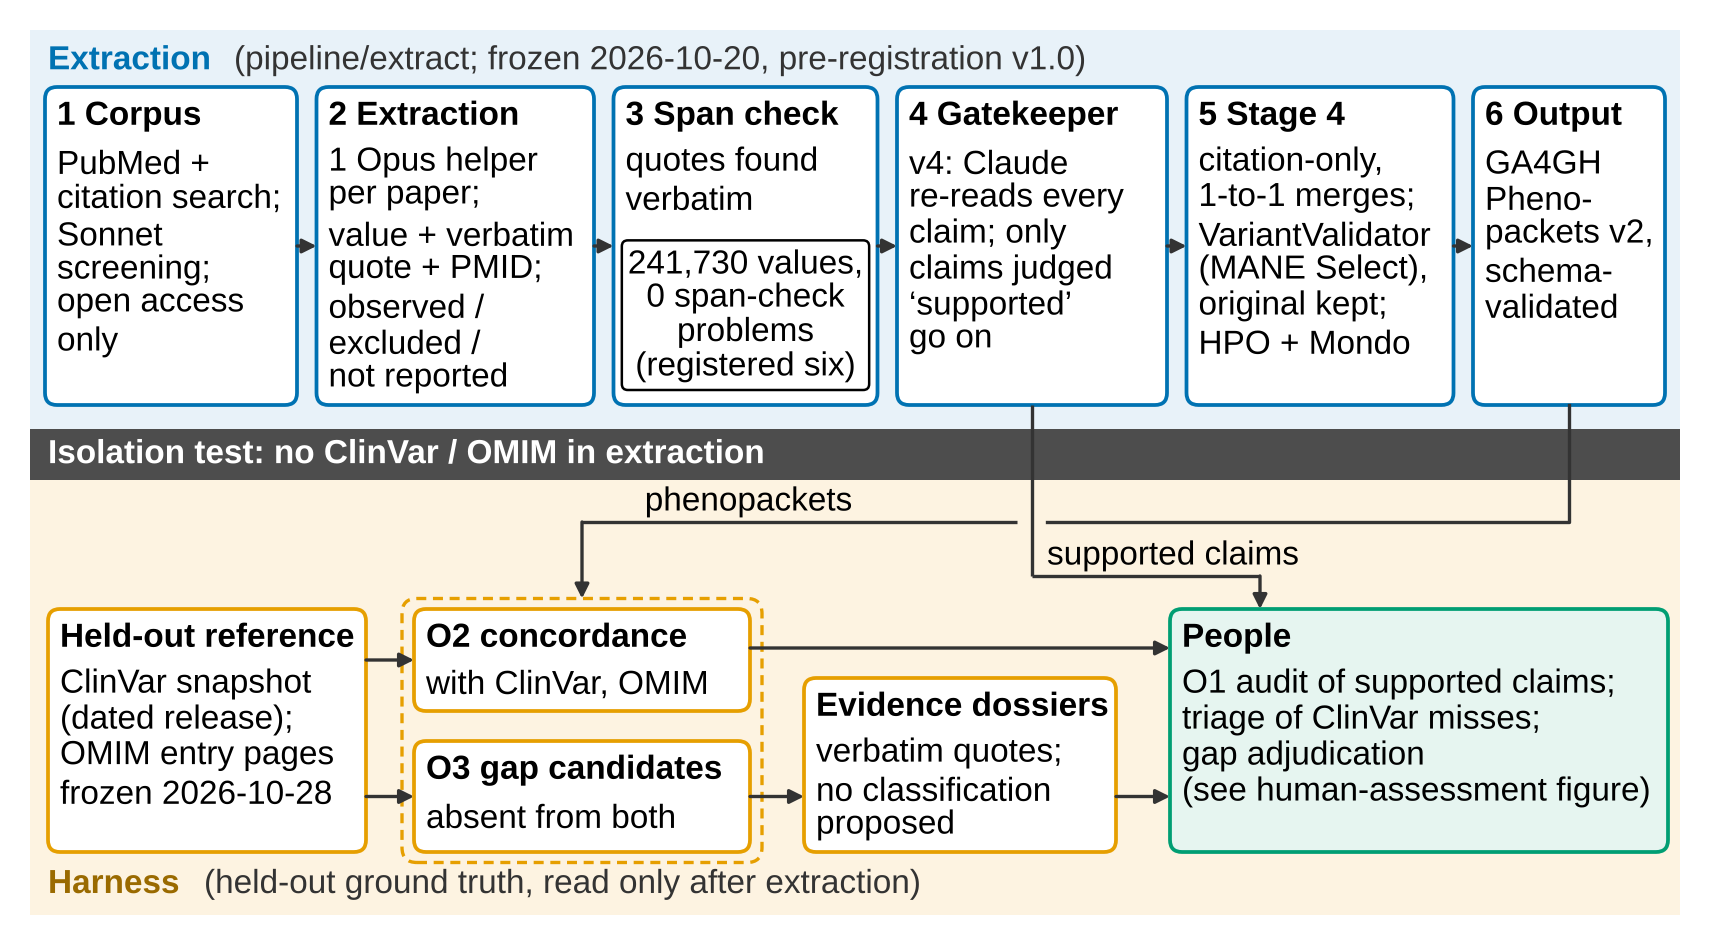
\includegraphics[width=0.66\linewidth]{figures/fig_pipeline_overview_v1.png}
\end{center}
\caption{GP-RareLink pipeline and its database-held-out evaluation. Top: extraction, frozen with pre-registration v1.0 on 2026-10-20; an isolation test keeps ClinVar and OMIM out. Bottom: the harness reads a dated ClinVar snapshot and OMIM pages frozen on 2026-10-28 only after extraction, to score concordance (O2) and list gap candidates (O3) with dossiers that propose no classification; people audit supported claims (O1), triage ClinVar misses and adjudicate candidates.}
\label{fig:pipeline}
\end{figure}

\begin{table}[t]
\caption{The twelve diseases (inheritance; papers in the main run). Only the registered six form the registered study; the extension five (separately pre-registered) and Majeed (exploratory) are reported beside it. Mondo identifiers and transcripts are in Appendix~\ref{app:registered}.}
\label{tab:diseases}
\begin{center}
\scriptsize
\begin{tabular}{llr@{\hspace{1.5em}}llr}
\toprule
\multicolumn{3}{l}{Registered six} & \multicolumn{3}{l}{Extension five and exploratory Majeed (not registered)} \\
\midrule
A20 haploinsufficiency, HA20 (\emph{TNFAIP3}), dev. & AD & 85 & Blau syndrome (\emph{NOD2}) & AD & 68 \\
SSADH deficiency (\emph{ALDH5A1}) & AR & 40 & Familial LCAT deficiency (\emph{LCAT}) & AR & 50 \\
Tangier disease (\emph{ABCA1}) & AR & 31 & GAMT deficiency (\emph{GAMT}) & AR & 23 \\
Leukocyte adhesion def.\ I, LAD-I (\emph{ITGB2}) & AR & 42 & Arterial tortuosity, ATS (\emph{SLC2A10}) & AR & 34 \\
Alexander disease, AxD (\emph{GFAP}) & AD / de novo & 69 & PAPA syndrome (\emph{PSTPIP1}) & AD & 34 \\
Danon disease (\emph{LAMP2}) & XLD & 83 & Majeed syndrome (\emph{LPIN2}); exploratory & AR & 24 \\
\bottomrule
\end{tabular}
\end{center}
\end{table}

\paragraph{Diseases, corpus and access.} The registered study is the six diseases of the frozen pre-registration \citep{elhani2024_ha20_177,didiasova2020_ssadh_update,koseki2021_tangier_review,almarzanovoa2018_lad1_review,brambatti2019_danon_gender}. Five reserve diseases \citep{wouters2014_blau,vitali2022_lcat,stockleripsiroglu2014_gamt,beyens2018_ats,hajialigol2022_papa} were run under an extension addendum committed before their extraction; Majeed syndrome \citep{ferguson2021_majeed} failed that addendum's floor (10 eligible open reports, under 15), was searched more widely and run on 24 documents as an exploratory disease. The corpus came from PubMed (inception to 2026-10-18/19 for the registered six, 2026-11-14 for the extension) with gene, disease names and a case filter, plus backward citation search through Europe PMC \citep{Rosonovski2023EuropePmc}. No database citation list seeded a corpus except HA20's pilot corpus (92 of 160 papers, tagged; O2 is reported with and without them). Sonnet helpers screened with logged reasons (full-text inclusion needed a script-checked quote); a PI check agreed with 14 of 15 inclusions (exact 95\% CI 68--100\%) and 5 of 5 exclusions (48--100\%). Access is open only: PMC, Europe PMC and Unpaywall copies, no institutional access, no pages behind a bot check; supplements capped at 60,000 characters per file. Every registered disease cleared the substitution floor of 15 eligible reports; natural-history comparator papers are held out.

\paragraph{Extraction.} SLIDERS \citep{joshi2026_sliders} is run as a home-built version by Claude Code helper agents on the funded claude.ai account, not the public code. One Claude Opus helper per paper reads only its paper, the instructions, the schema and the rules, with no web access and an instruction to use nothing it remembers about the paper (run provenance in the Reproducibility Statement). Four files were pinned at the freeze; per disease a script swaps only the disease name, gene, schema path and a 20-item checklist. Every value carries the PMID and a verbatim quote, confirmed by a deterministic span check; ``not reported'' carries no quote, and a value without a quote is not emitted, so complete quote coverage is a property of the pipeline rather than a finding. Normal findings are recorded as the excluded abnormality, variant fields come only from statements about this person, and stacked multi-patient cells are not read by position. One gap was frozen on purpose: extraction has no rule for hedged wording, so hedged statuses are removed by the gatekeeper and end as ``not reported''.

\paragraph{Gatekeeper.} Gatekeeper v4 is a separate Claude Opus read, one helper per chunk of up to 350 claims. It asks whether the quote entails the value for the person the row is about \citep{rashkin2023_ais}, records whom the quote is about (this person, a named group, the cohort, another person, the paper, unclear) and returns supported, partially supported, unsupported or span not found; no value is exempted by script matching, and phenopackets keep only supported claims. ``Unsupported'' below counts unsupported and span not found; ``not fully supported'' adds partially supported. Because a model judging its own family's output can be biased \citep{zheng2023_llm_judge}, the gatekeeper's share is a screen evaluated against human labels, never an error rate.

\paragraph{Records.} People are merged only on an explicit one-to-one citation to an earlier report (a sex-and-onset route made all 6 false merges of 93 in the pilot and was dropped). VariantValidator 4.0.1 \citep{freeman2018_variantvalidator} normalizes variants to HGVS \citep{hart2024_hgvs2024} on MANE Select \citep{morales2022_mane}, keeping the paper's original string; only its normalization fields enter the pipeline. Where a gene has alternative coding exons (LAMP2, GFAP), the paper's own exon label chooses the transcript, else no genomic key is given (a post-freeze change); for Blau, a reference mismatch on MANE triggers one retry on legacy NM\_022162.3. Features are bound to HPO (2026-09-01) and diseases to Mondo (2026-10-06) by name, never by OMIM cross-reference, and one Phenopacket v2 \citep{jacobsen2022_phenopacket_schema} per identity is validated \citep{danis2023_phenopacket_tools}. Post-freeze changes are logged deviations (Appendix~\ref{app:deviations}).

\paragraph{Held-out ground truth and outcomes.} An automated test fails if any reference path or the tokens ``clinvar'', ``omim'' or ``harness'' appear in the extraction code; snapshots live outside the repository, and database citation seeds, annotation files, LitVar's ClinVar links, database fields in VariantValidator responses and comparator papers are kept out. References: ClinVar release 2026-10-12 (read 2026-10-19) for the registered six and of 09~Nov~2026 for the rest; OMIM's entry pages frozen by the PI on 2026-10-28 (clinical synopses not frozen); HPO annotations on the harness side only (Appendix~\ref{app:registered}). \textbf{O1}: 250 claims sampled from all gatekeeper-supported claims, stratified by disease, seeded, drawn before any concordance; raters never see the gatekeeper's verdict, and an unverifiable value counts as unsupported. O1 thus measures error in the released records, after the screen; claims the gatekeeper removed are outside it. Rule~C passes if at most 4 are unsupported; P(pass) is 0.99, 0.89, 0.68, 0.44 and 0.13 at true rates of 0.5\%, 1\%, 1.5\%, 2\% and 3\%, and with 0, 1 or 2 unsupported the exact two-sided 95\% upper bound is 1.46\%, 2.21\% or 2.86\%, so a pass does not prove a rate below 2\%. \textbf{O2}: tier~1 = same GRCh38 allele, tier~2 = same protein change for papers with no cDNA; HGVS recall = share of ClinVar's (PMID, variant) pairs for extracted PMIDs that the run extracted from that PMID, so recall is computed only on papers with open full text; overlap = share of extracted tier-1 alleles in ClinVar (not precision); no threshold. \textbf{O3}: a gap candidate is a gatekeeper-supported tier-1 allele absent from ClinVar and (registered six) from OMIM; it is a candidate, not a finding, until adjudicated; submissions will use ClinVar's \emph{curation} method. \textbf{O4}: literature frequencies against held-out cohorts with a publication-cluster bootstrap \citep{Efron1979BootstrapMethods} (2,000 resamples, seed 7425; records with a disease term, comparator members removed), plus a memorization probe. \textbf{O5}: expert minutes per accepted record, and Claude against an open-weight model under an identical scaffold. Intervals: Wilson \citep{Wilson1927ProbableInference} for proportions, exact Clopper--Pearson \citep{Clopper1934UseConfidence} for audit and gatekeeper shares.

\paragraph{Human assessment.} Since 2026-11-15 the audit is done by volunteer raters in rotating groups after a calibration round with a floor, replacing two fixed raters and a tie-breaker (design in Appendix~\ref{app:planning}). Nine raters, none identified, rate 40 calibration claims that the PI labelled (20 unsupported, 20 supported, chosen by a rule fixed before any label and amended twice before any rater saw anything); only a rater who catches at least 15 of the 20 unsupported and passes at least 18 of the 20 supported serves as a registered rater. Each audit claim is read by 3 raters, with a registered pair and tie-breaker per claim and rule~C unchanged; Cohen's $\kappa$ \citep{Cohen1960CoefficientAgreement} is reported per pair. Misses are triaged and candidates adjudicated under ACMG/AMP \citep{richards2015_acmg} by 2 raters each, a third where they differ. The PI then chooses Plan A (registered six: 250 claims, 50 misses, 214 candidates) or Plan B (all twelve: 527, 146, 269).
%%%%%%%%% METHOD %%%%%%%%%

\section{Experiments}
\label{sec:experiments}
%%%%%%%%% EXPERIMENTS %%%%%%%%%
Sections~\ref{sec:prov}--\ref{sec:o4o5} report the registered six only; Section~\ref{sec:beside} reports everything else.

\subsection{Registered six: provenance and scale}
\label{sec:prov}
\begin{table}[t]
\caption{Registered six (frozen pipeline, runs of 2026-10-20). Span-check problems are 0 in every row. Gatekeeper shares (counts; exact 95\% CI) are a screen by a second model read, not error rates. HA20 is the development disease.}
\label{tab:registered}
\begin{center}
\resizebox{\linewidth}{!}{%
\begin{tabular}{lrrrrllr}
\toprule
Disease & Papers & Indiv.\ rows & Values quoted & Claims judged & Unsupported & Not fully supported & Phenopackets (interp.) \\
\midrule
HA20 (dev.) & 85 & 811 & 67,863 & 23,129 & 0.20\% (46; 0.15--0.27) & 1.93\% (446; 1.75--2.11) & 769 (499) \\
SSADH & 40 & 421 & 31,370 & 9,759 & 0.38\% (37; 0.27--0.52) & 2.86\% (279; 2.54--3.21) & 363 (174) \\
Tangier & 31 & 235 & 16,762 & 4,830 & 0.31\% (15; 0.17--0.51) & 4.49\% (217; 3.93--5.12) & 235 (53) \\
LAD-I & 42 & 508 & 36,280 & 10,864 & 0.43\% (47; 0.32--0.57) & 3.47\% (377; 3.13--3.83) & 508 (299) \\
AxD & 69 & 463 & 40,773 & 14,403 & 0.27\% (39; 0.19--0.37) & 3.55\% (512; 3.26--3.87) & 456 (255) \\
Danon & 83 & 510 & 48,682 & 17,963 & 0.61\% (110; 0.50--0.74) & 3.07\% (552; 2.83--3.34) & 505 (212) \\
\midrule
Five confirmatory & 265 & 2,137 & 173,867 & 57,819 & \textbf{0.43\% (248; 0.38--0.49)} & 3.35\% (1,937; 3.20--3.50) & -- \\
All six & 350 & 2,948 & 241,730 & 80,948 & \textbf{0.36\% (294; 0.32--0.41)} & 2.94\% (2,383; 2.83--3.06) & 2,836 (1,492) \\
\bottomrule
\end{tabular}}
\end{center}
\end{table}

All 241,730 asserted values have a quote the span check found verbatim (Table~\ref{tab:registered}); this confirms the pipeline invariant and shows no quote was altered, not that the values are right. 2,948 rows became 2,836 identities through 112 citation merges (SSADH's 58 all join a preprint and its journal version); all 2,836 phenopackets are schema-valid, 1,492 carry an interpretation, and they hold 12,679 observed and 3,371 excluded HPO terms; 485 (17\%) hold identity fields only. HPO binding covers 84\%--93\% of feature rows and cDNA normalization ranges from 78.9\% (AxD) to 96.7\% (HA20) (our sources differ on the denominators, so we give percentages only); ``not reported'' far outnumbers values. Identities are an upper bound on people: 9 of 38 repeat papers differ in individual count, and if all 19 proposed same-person groups (unmerged, awaiting a person) were confirmed, 3.8\% of HA20 identities would collapse and 0.2\%--1.2\% elsewhere, itself a lower bound because only the gap candidates' papers were examined. A 10\% repeat (38 papers, seed 20261020, no gatekeeper) agreed on 97\%--100\% of checklist cells and on variant keys at 0.92--1.00 in four diseases (0.83 Tangier, 0.86 Danon, one paper each using a different notation), but only 0.43--0.71 on free-text feature rows; the individual-count differences come from scope calls on relatives and cited patients, the weakness reported for proband counting elsewhere \citep{murugan2026_reasoning_llm_ps4}.

\subsection{Accuracy evidence so far: two pilot audits, and a screen}
\label{sec:accuracy}
\begin{figure}[t]
\begin{center}
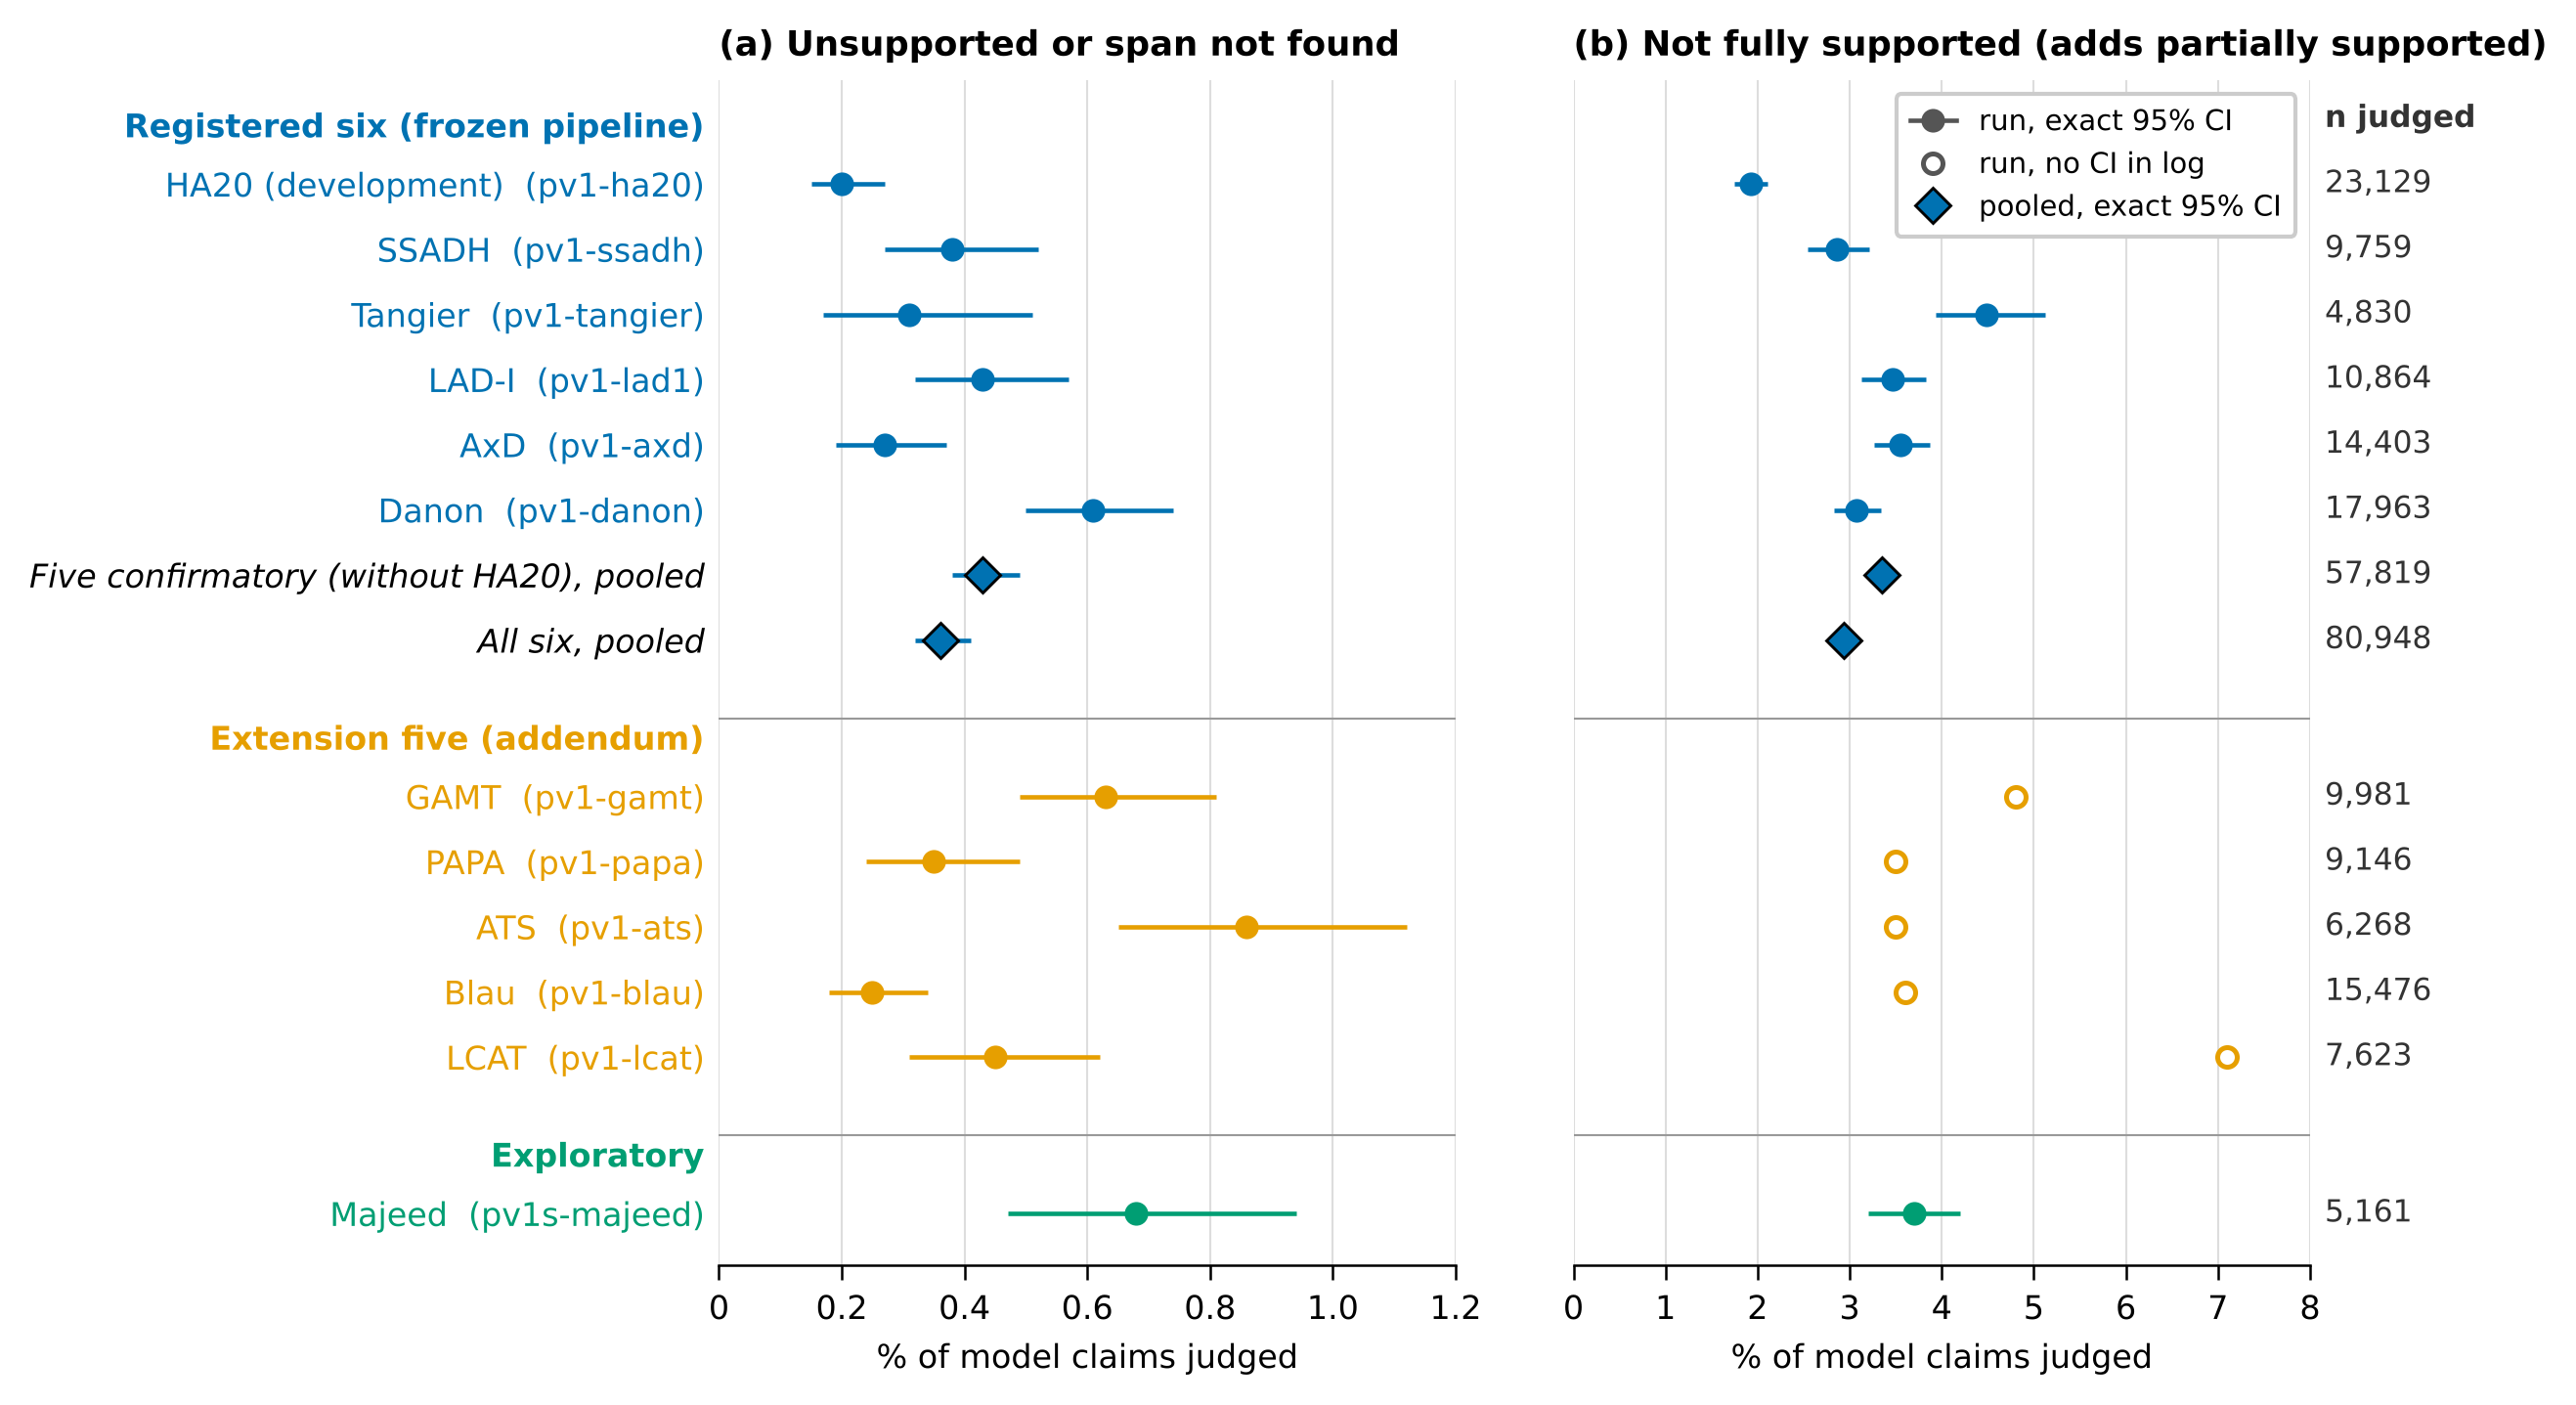
\includegraphics[width=0.60\linewidth]{figures/fig_gatekeeper_by_run_v1.png}
\end{center}
\caption{Gatekeeper shares per main run: (a) unsupported or span not found; (b) not fully supported (adding partially supported); exact 95\% CIs where available (open circles: none in the log); claims judged at right. Registered six with pooled five confirmatory and all six (diamonds); extension five and Majeed apart; addendum not shown. A screen, not an error rate: no comparison with the 2\% target is possible.}
\label{fig:gatekeeper}
\end{figure}

\paragraph{Human audits (pilot, pre-freeze).} The only human ratings of extracted claims are two pilot audits on HA20 by one rater: 6.0\% (3/50; exact 95\% CI 1.3\%--16.5\%) and 6.3\% (3/48; 1.3\%--17.2\%) unsupported, both above the pilot's own 4\% gate. Each exposed an error class (variant fields taken from a group statement; ages read by position from stacked cells) for which a rule was frozen; variant fields were 0 of 20 unsupported in the re-audit against 3 of 20 before, but the frozen pipeline has not been re-audited. Without the 3 claims the rater could not verify, the re-audit found 0 of 45. Both audits used earlier pipeline versions, and labels in the second-look tab are not independent of the gatekeeper's reasons.

\paragraph{The gatekeeper is a low-sensitivity screen.} In those audits earlier gatekeeper versions flagged only 2 of the 6 and 1 of the 4 claims the person rejected (no false flags) and found 0.036\% and 0.34\% unsupported against the person's 6.0\% and 6.3\%. Its registered shares (Figure~\ref{fig:gatekeeper}) are 0.43\% (248/57,819; 0.38--0.49) pooled over the five confirmatory diseases and 0.36\% (294/80,948) with HA20; it removed 1,060 claims before the phenopackets were built. They are what a second model read catches, not error rates. The PI's calibration labels also disagree with it in both directions: of 65 candidates it removed he labelled 34 supported, 26 unsupported, 4 not verifiable and 1 quote not in paper; of 34 it kept, 30 supported, 3 unsupported, 1 not verifiable (candidates chosen for variety and labelled by one person, so not rates either). What the screen's removals show is where extraction fails (measured by counting verdicts): in five of six diseases the three worst papers hold half or more of the unsupported claims (Danon's three hold 60 of 110; one paper gave a proband's variant and diagnosis fields to eight family carriers, 35 claims); the commonest unsupported field in five diseases is a variant row's gene symbol quoted from a sentence about someone else; then hedged wording recorded as observed or excluded (the frozen gap) and cohort statements applied to individuals.

\paragraph{O1, the primary outcome (pending).} 250 of the 78,564 gatekeeper-supported claims (HA20 72, SSADH 30, Tangier 15, LAD-I 33, AxD 44, Danon 56) were drawn on 2026-10-20 with seed 40250, before any concordance. The audit found \HR{o1_unsupported_n} of 250 unsupported (\HR{o1_unsupported_pct}; exact 95\% CI \HR{o1_unsupported_ci}); rule~C: \HR{o1_rule_c}; Cohen's $\kappa$ over rater pairs: \HR{o1_kappa_range}; share of human-unsupported claims the gatekeeper had also removed: \HR{o1_gatekeeper_sens} (by disease in Appendix~\ref{app:o1o3}). This result decides whether the frozen pipeline meets the registered target. Because O1 samples the released records, the gatekeeper's low sensitivity enters it directly: a pipeline whose true residual rate is 2\% passes rule~C with probability 0.44, and one at 3\% with probability 0.13. Whatever the result, it is reported as computed; any fix would be a logged deviation, re-run and reported beside the registered result, which stays primary.

\subsection{O2: concordance with ClinVar}
\begin{figure}[t]
\begin{center}
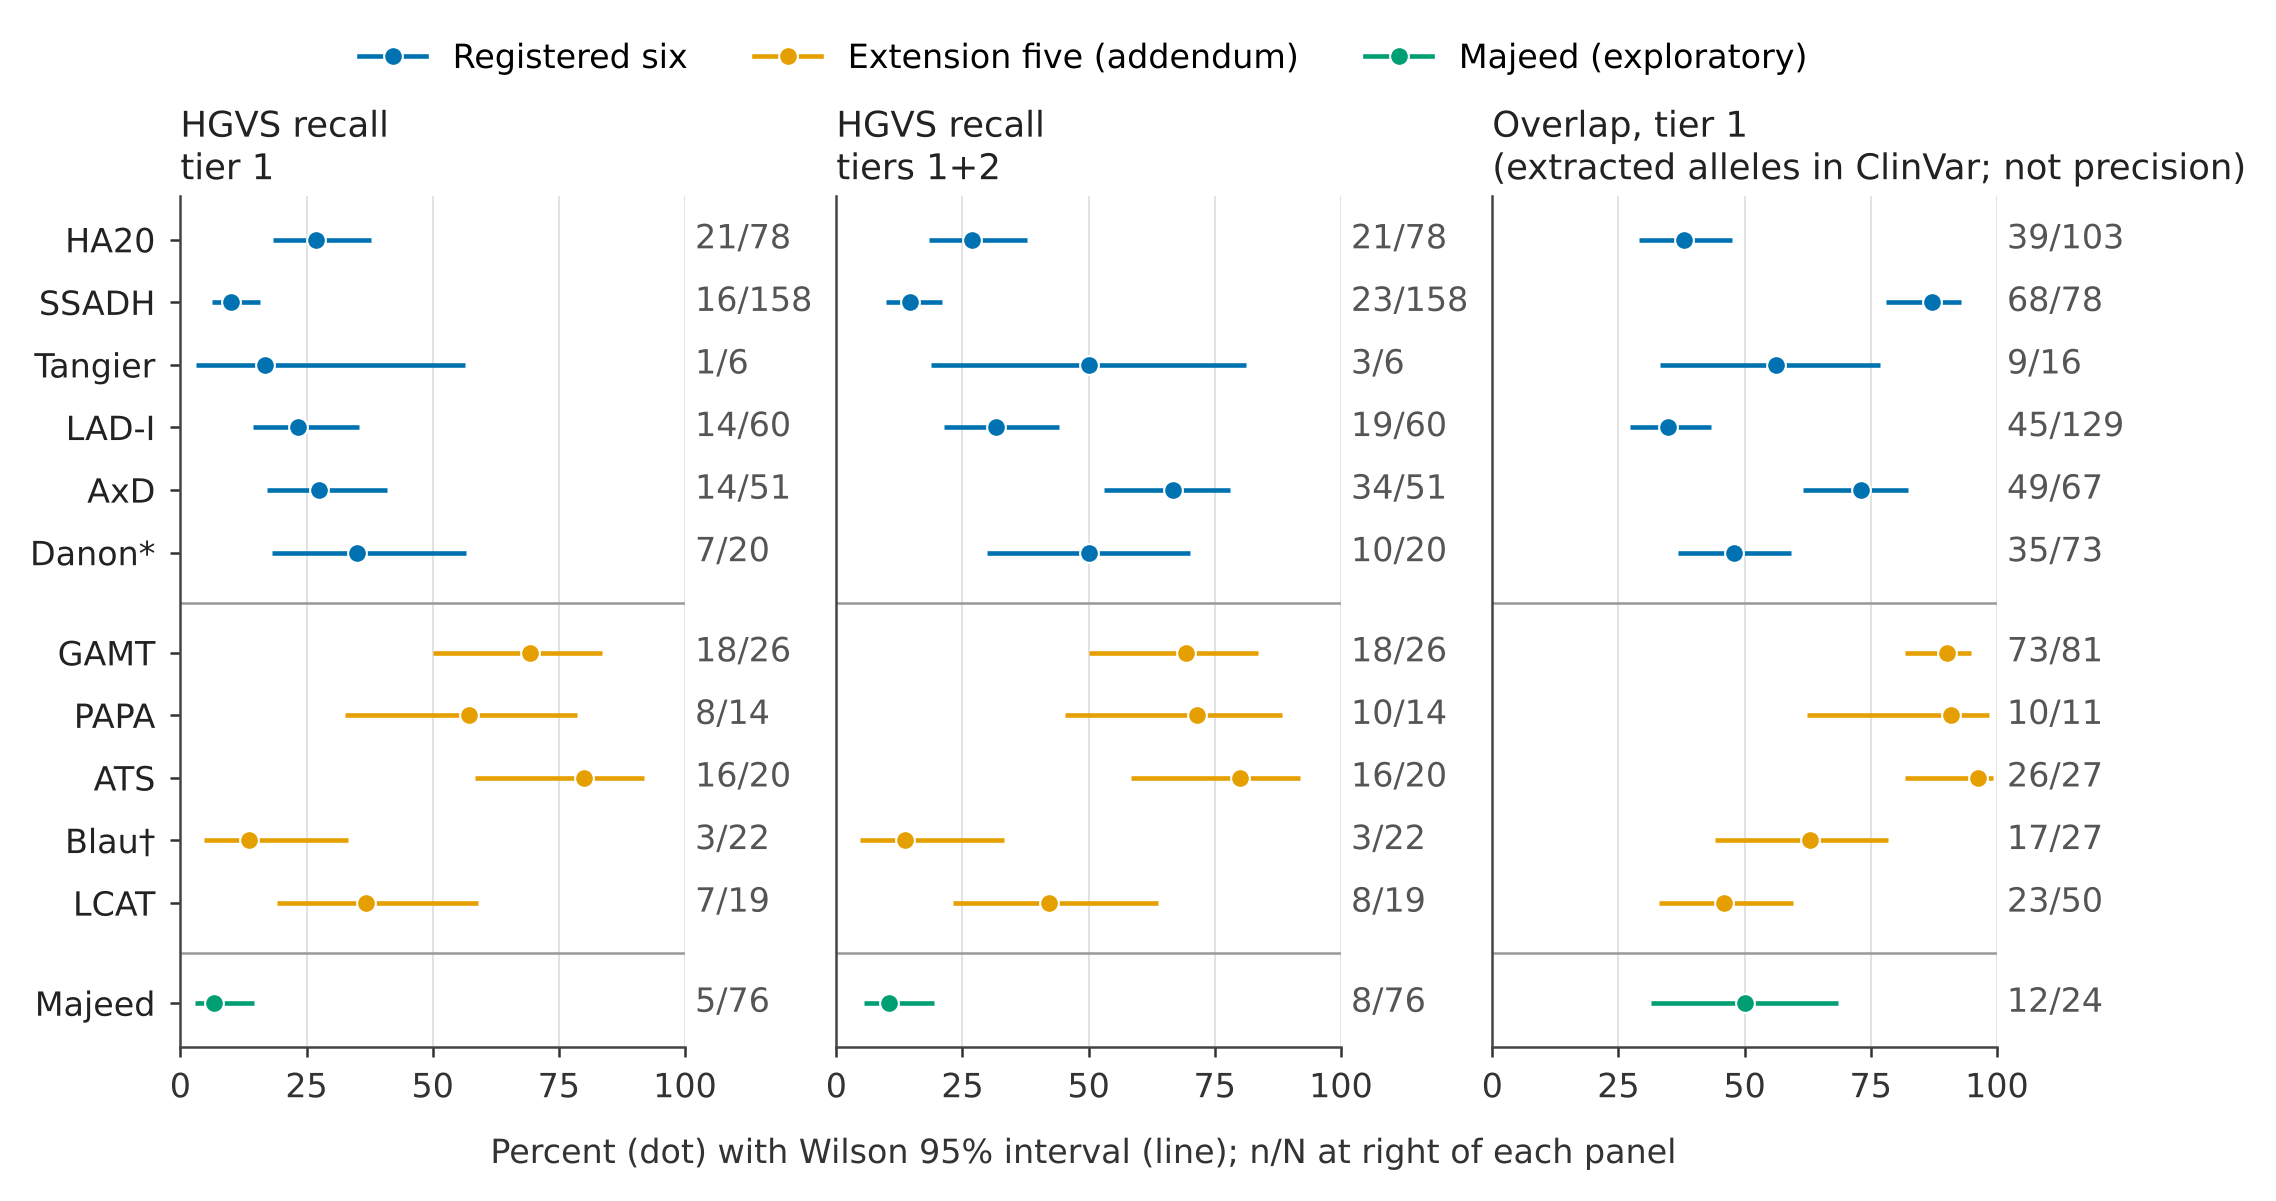
\includegraphics[width=0.66\linewidth]{figures/fig_o2_concordance_v1.png}
\end{center}
\caption{ClinVar concordance (O2): HGVS recall at tier~1 (same GRCh38 allele) and tiers 1+2 (adding protein matches for papers with no cDNA), and tier-1 overlap (extracted alleles in ClinVar; not precision); Wilson 95\% intervals, n/N at right. Registered six, extension five and Majeed use different snapshots and are not pooled. *~Danon predates the isoform re-normalization of 2026-10-28. \dag~Blau with the legacy NOD2 transcript retry (4.5\%, 1/22, at tier~1 under the registered rule). No threshold applies.}
\label{fig:o2}
\end{figure}

The extracted gene matches the disease gene in 97.9\%--100\% of registered variant rows. HGVS recall (Figure~\ref{fig:o2}) is low, 10.1\%--35.0\% at tier~1 and 14.6\%--66.7\% with protein matches, over ClinVar citation pairs of extracted papers only (HA20 78, SSADH 158, Tangier 6, LAD-I 60, AxD 51, Danon 20), so the denominators are small for Tangier and Danon. Every miss counts as discordant until triaged. \emph{Measured:} misses sit in single papers: the founding HA20 paper (PMID 26642243) holds 52 of HA20's 57; a LAD-I mutation update (22134107) 37 of 41; in SSADH two papers (14635103, 33203024) 68 and 53 of 135; and for 28 of the 50 sampled misses a script found no mention of the variant's position or residue in the paper text. \emph{Hypothesised, for triage to test:} that ClinVar cites the HA20 founding paper for variants it does not describe; that an SSADH table was scrambled in conversion (helper-reported, unverified); that the 53 misses of the other SSADH paper, an in-vitro study with no patients, are variants with no person to extract. The triage will give \HR{o2_triage_breakdown}. A split of recall by kind of ClinVar citation has not been computed. Overlap is 35\%--87\% and is not precision. Classification agreement among stated values is 59\%--92\%, and the disagreements run one way (authors P/LP, ClinVar VUS), as expected in advance; this is not evidence about extraction error. Against published catalogues, recall restricted to source papers in the corpus is 9 of 9 (HA20) and 54 of 56 (AxD; the two misses are notation), against 90.6\% (29/32) and 53.8\% (91/169) unrestricted: the restricted figures measure reading, the unrestricted mostly access. Full tables, with and without ClinVar-cited papers, are in Appendix~\ref{app:o2}.

\subsection{OMIM as a human-curated holdout, and the access constraint}
\begin{figure}[t]
\begin{center}
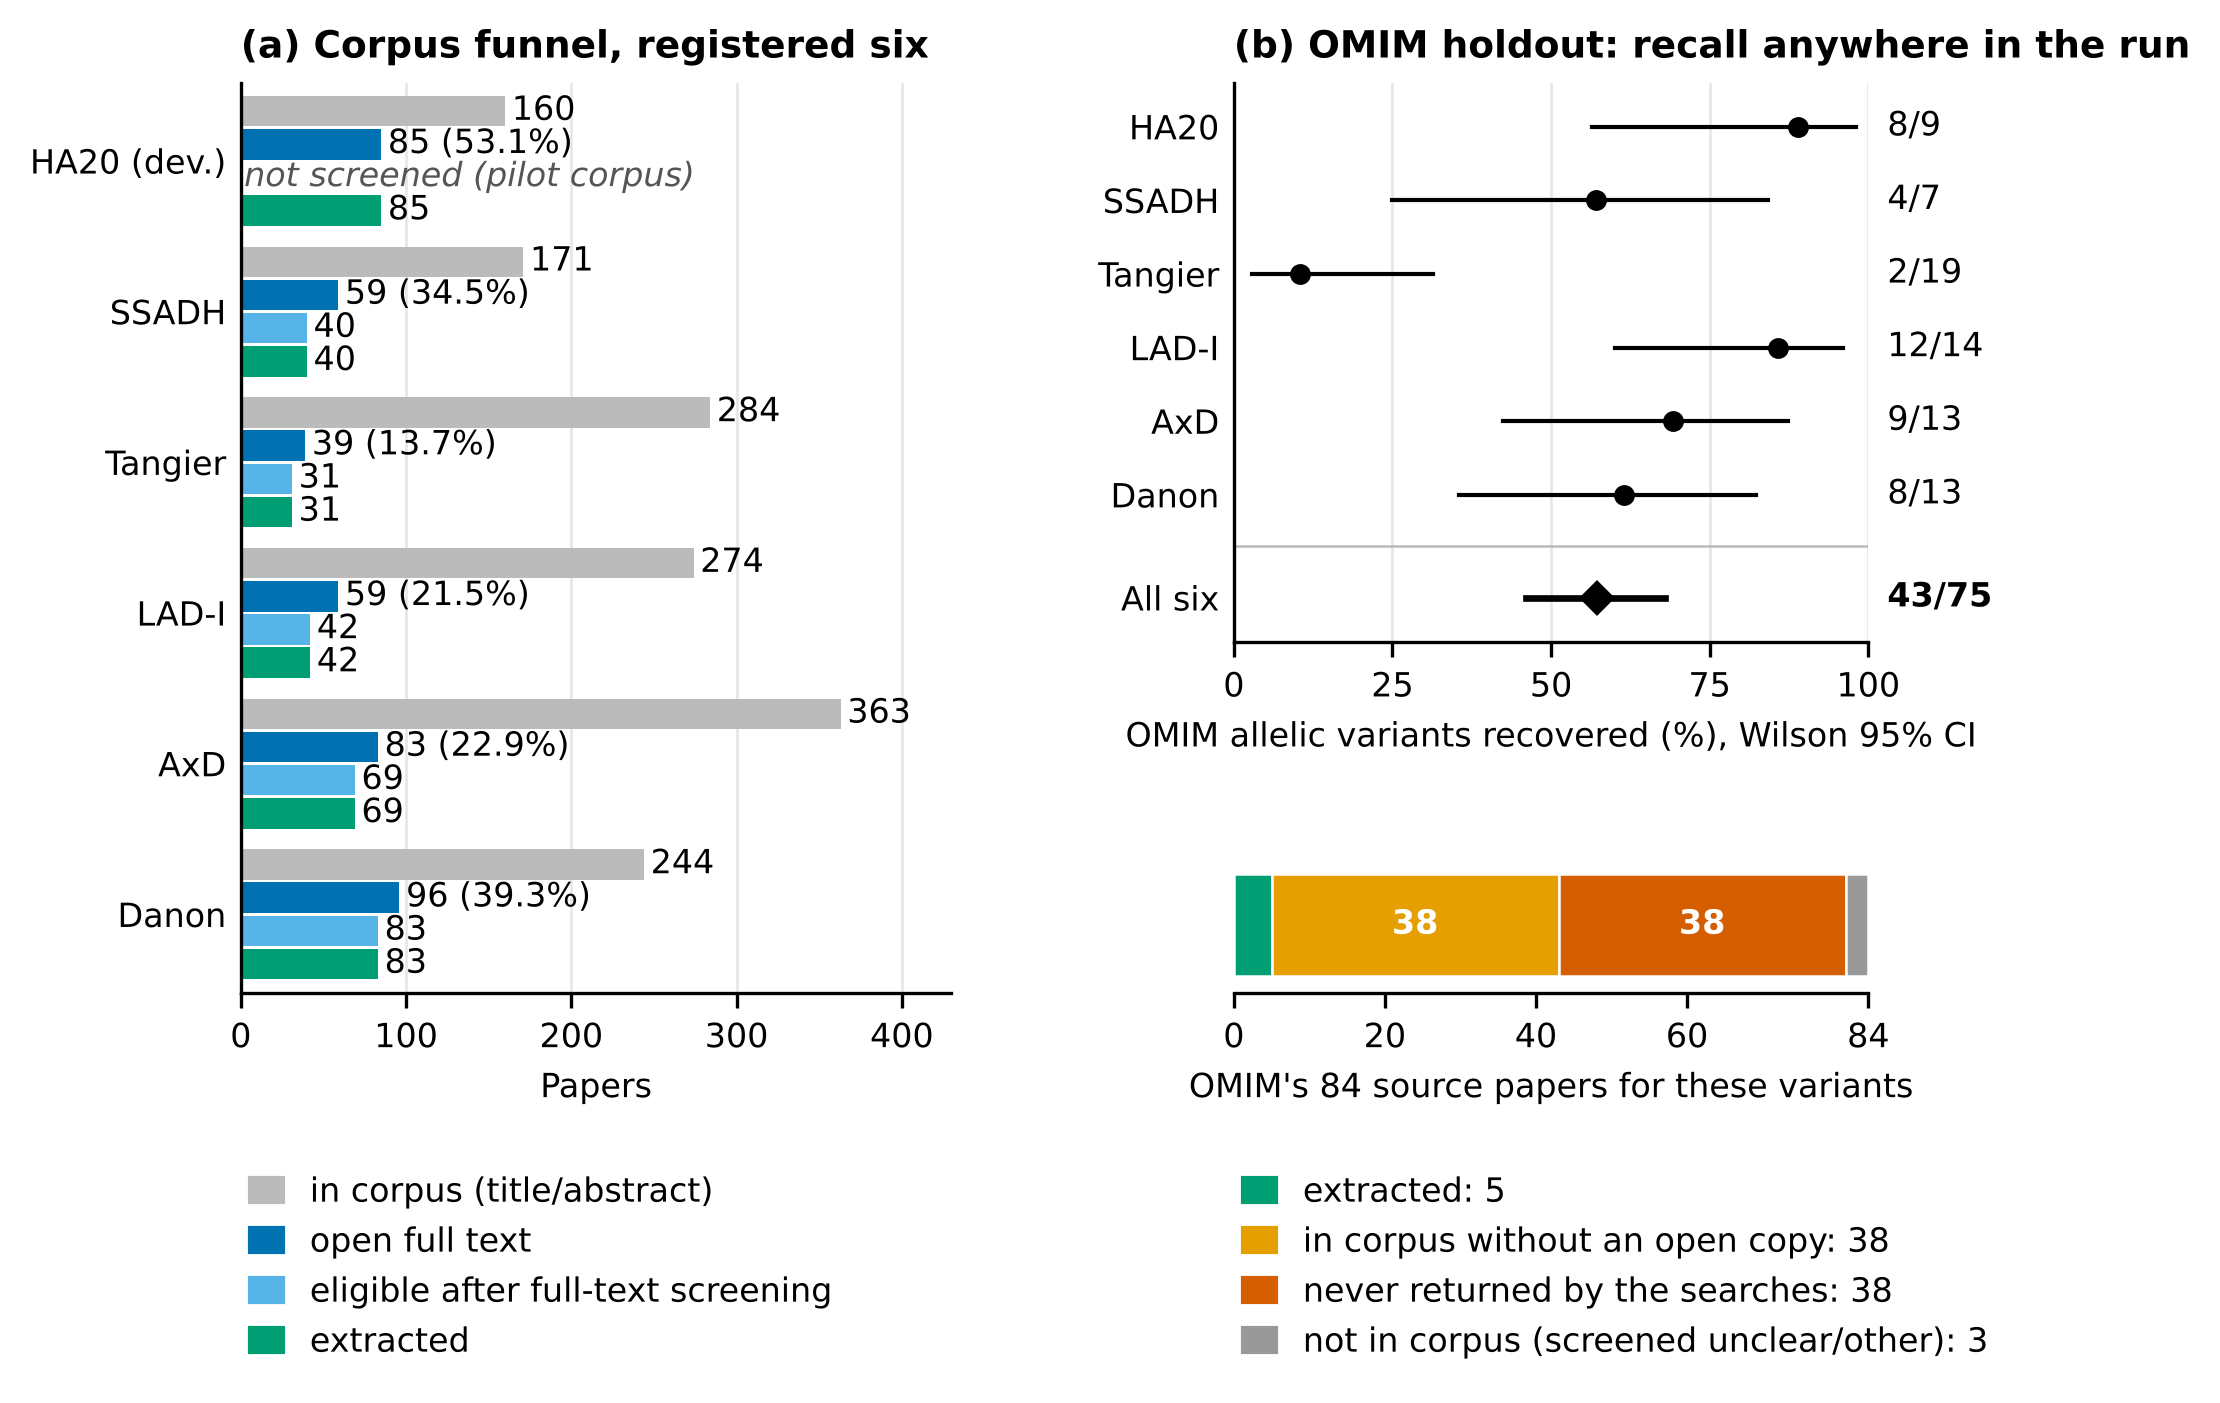
\includegraphics[width=0.60\linewidth]{figures/fig_access_constraint.png}
\end{center}
\caption{(a) Corpus funnel, registered six (title/abstract corpus; open full text; eligible; extracted). (b) OMIM allelic variants recovered anywhere in the run (tiers 1+2), Wilson 95\% intervals: 43 of 75 pooled (57.3\%, 46.1--67.9); below, where OMIM's 84 source papers for them sit (5 extracted, 38 in corpus without an open copy, 38 never returned by the searches, 3 not in corpus).}
\label{fig:access}
\end{figure}

Open full text exists for 421 of 1,496 registered corpus papers (28\%), from 13.7\% (Tangier) to 53.1\% (HA20) (Figure~\ref{fig:access}a), in line with the partial reach of open access \citep{Piwowar2018StateOa}; paywalled papers are not a random subset, so every count here is a lower bound on a selected literature. The runs recover 57.3\% (43/75; 46.1--67.9) of OMIM's allelic variants, 58.7\% (44/75) counting a notation-level match, but 10.5\% (2/19) for Tangier, whose 17 misses all have no source paper in the run (Figure~\ref{fig:access}b). \emph{Measured:} of OMIM's 84 source papers for these variants only 5 were extracted, 38 are in the corpus without an open copy and 38 were never returned by the searches; where the source paper was extracted, 8 of 14 variants were recovered from it (misses: a table scrambled in conversion, and two variants stated only in prose). Our reading of this, that literature access bounds recovery more than reading does, rests on these counts; reading accuracy on OMIM's own papers rests on 14 variants. At patient level, judged by Claude and not by a panel member, 12 of 23 comparisons agree, 7 partially, 4 are missed and none contradicts OMIM. OMIM is fallible too (two allelic variants link to non-matching ClinVar records; legacy numbering), and only its variant half is assessed.

\subsection{O3: gap candidates, none yet shown to be real}
\begin{table}[t]
\caption{Gap candidates by study (stage~1). Only the first row is the registered study. The last row holds pending results. Nothing has been adjudicated or submitted.}
\label{tab:o3}
\begin{center}
\scriptsize
\begin{tabular}{lrrrr}
\toprule
Study & Candidates & Withdrawn & Left for the panel & Individuals behind them \\
\midrule
Registered six & 215 & 1 & 214 & 372 \\
Extension five (not registered) & 45 & 2 & 43 & 72 \\
Majeed (exploratory) & 12 & 0 & 12 & 22 \\
All twelve & 272 & 3 & 269 & -- \\
\midrule
\multicolumn{5}{p{0.8\linewidth}}{Pending: adjudicated \HR{o3_adjudicated}; accepted \HR{o3_accepted}; by class \HR{o3_class_split}; records prepared \HR{o3_submissions}} \\
\bottomrule
\end{tabular}
\end{center}
\end{table}

The registered six give 215 candidates, 214 after one withdrawal (Table~\ref{tab:o3}); all 215 were still absent by allele from the next ClinVar release, and 214 are absent from OMIM. No candidate is yet shown to be a real gap, and three of 272 across all twelve diseases have already proved to be placement artefacts (a Danon deletion on the wrong LAMP2 isoform; a Blau and an LCAT variant read on the wrong transcript). LAD-I's 82 registered candidates need most care: 66 come only from papers ClinVar cites for \emph{ITGB2} and 34 only from reviews, so a numbering slip is as likely as a true gap. Dossiers for all 215 hold 4,725 quotes, all verbatim, on case count, segregation, de novo status, functional evidence and variant type, and propose no classification; population frequency is left to the panel because gnomAD \citep{Karczewski2020MutationalConstraint} is not reachable from the environment. 152 of 215 carry a triage flag (most often ``possible same person twice'', 77). Adjudication will decide how many of the 214 are true gap variants with phenotype evidence (\HR{o3_accepted}).

\subsection{O4 and O5}
\label{sec:o4o5}
\paragraph{Memorization and bias.} On 180 papers (10 after Claude's June 2026 cutoff, 51 recent, 119 older), closed-book recall and guided completion of a 50-word opening, scored with ROUGE-L \citep{Lin2002ManualAutomatic} and 5-gram overlap, were run identically on both models. Claude claimed specific recall for 4 older papers (phenotypes only); its 4 variant hits were guesses of recurrent variants. Neither model reproduced the papers' variants or text, but the after-cutoff stratum has 10 papers and black-box probes can miss memorization that changes extraction. Frequency deviation has not started (no comparator sheet filled); primary denominators were fixed first (records with a disease term, comparator members removed: SSADH 363 $\rightarrow$ 311 $\rightarrow$ 196, HA20 769 $\rightarrow$ 447 $\rightarrow$ 438, Danon 505 $\rightarrow$ 322). Deviations: \HR{o4_deviation}.

\paragraph{Claude against an open-weight model.} DeepSeek-V4.1-Flash \citep{Deepseekai2026Deepseekv4Towards} ran on the same 125 papers (HA20, SSADH) with the same prompt and frozen files in a file-tool agent loop. Its quotes were not found for 3.86\% and 2.98\% of values (Claude 0.00\%), 2,003 and 991 values had no quote, and the gatekeeper judged 8.64\% and 6.14\% of its claims unsupported (Claude 0.20\% and 0.38\%), 2.28\% and 2.03\% among claims with a quote. HGVS recall overlaps within intervals (HA20 26.9\% vs 19.2\%; SSADH 14.6\% vs 15.2\%). Median cost per paper was \$0.07 against Claude's estimated \$1.08 and \$1.19, and median time 20.9 and 19.2 minutes against 2.9. The judge is Claude; empty quotes were handled unevenly; the scaffold differed in stated ways; the scope is two diseases, one model, one provider (Appendix~\ref{app:secondary}). The registered blinded audit is pending: \HR{o5_openweight_audit}; expert minutes per accepted record: \HR{o5_minutes_per_record} (the only measured rating times are the pilot's 0.37 and 0.65 minutes per rating). Exploratory GPSEA maps \citep{rekerle2026_gpsea} with Benjamini--Hochberg correction \citep{Benjamini1995ControllingFalse} found no significant term in five diseases; Danon reproduces the published sex difference \citep{boucek2011_danon_natural_history}, a check on overlapping papers, not a replication.

\subsection{Beside the registered study: extension, exploratory disease and corpus addendum}
\label{sec:beside}
None of these results enters a registered figure. \emph{Extension five} (separately pre-registered before extraction; bias arm, open-weight comparison and OMIM check not extended): 209 papers, 1,617 valid phenopackets, gatekeeper 0.25\%--0.86\%, tier-1 recall 13.6\% (Blau, where 17 of the 19 remaining misses are protein-only descriptions in legacy NOD2 numbering) to 80.0\% (ATS), and 43 candidates left for the panel. \emph{Majeed} (exploratory; its ClinVar comparison and candidates were read before its 27-claim audit sample was drawn): 24 documents, 158 phenopackets, gatekeeper 0.68\% (35/5,161), tier-1 recall 6.6\% (5/76), 12 candidates; outputs of 6 documents that are not openly licensed are held back. \emph{Corpus addendum} (free copies found after the freeze, PDF-converted with Docling \citep{Auer2024DoclingTechnical}; not deduplicated or matched to the registered runs; no concordance yet): 82 papers, 561 phenopackets; batch~1 (23 papers) 2.5\% unsupported, mostly Tangier (60/1,262) from 1970s group statements applied to named people; batch~2 (59 papers) 0.4\%, or 0.8\% counting strictly 45 softened ``other person'' verdicts. Pending: audits \HR{o1x_unsupported} of 250 (extension) and \HR{o1m_unsupported} of 27 (Majeed) under Plan B; addendum ratings \HR{add_b1_ratings} and \HR{add_b2_audit} (Appendix~\ref{app:beside}). Estimated spend: \$3,263.08 of \$45,000 (session readings of 2026-11-15, not billing; Appendix~\ref{app:budget}).
%%%%%%%%% EXPERIMENTS %%%%%%%%%

\section{Discussion and Limitations}
\label{sec:discussion}
Measured: complete provenance (by construction, and checked), valid three-state records from 350 papers, and held-out concordance and gap candidates. Not yet known, and to be decided by the pending results: whether released values meet the 2\% target (O1: \HR{o1_unsupported_pct}); how much of the low recall is extraction failure rather than citation, conversion or numbering (triage); which of the 214 registered candidates are true gaps (adjudication); and the bias deviations. The only human evidence, the pilot audits, sits an order of magnitude above the gatekeeper's shares, so those shares are not read as accuracy.

\paragraph{Limitations that change interpretation.} (1) No human-rated accuracy exists for the frozen pipeline; both pilot audits missed 2\% (one rater, HA20, earlier versions), their error classes are guarded against but not re-audited, and even a pass under rule~C leaves a true rate near 2\% unexcluded. (2) The gatekeeper is a same-family judge with measured low sensitivity (2 of 6, 1 of 4) and may favor Claude; its procedure was uneven in later runs (scripted verdict files, three addendum chunks judged once, one sentence judged both ways, softened verdicts, Majeed chunks changed on re-judging). (3) O1 samples only gatekeeper-supported claims, so it measures released records, not extraction before the screen. (4) Calibration rests on one person's reference labels, with a set rule amended twice after they were seen (before any rater saw anything), and the set is balanced 20/20, unlike the audit pool, so calibration catch rates do not carry over to audit prevalence. (5) Frozen extraction gaps remain (no hedge rule; relatives' variant fields from the proband's sentence; cohort statements applied to individuals) and drive higher addendum rates (batch~1 Tangier 4.8\%, batch~2 HA20 3.2\%). (6) HGVS recall is low and untriaged, and overlap is not precision. (7) Open access only (14\%--53\% per registered corpus), so the gap count is a lower bound on a non-random subset; 111 addendum papers and Majeed's founding reports remain unretrieved. (8) Deduplication is the weak point: besides the figures above, the pilot made 6 false merges of 93, the registered 50-merge hand check is not done, and addendum records are unmatched. (9) HA20 is the development disease (rules tuned on it; 92 of 160 papers ClinVar-seeded), so its figures flatter the pipeline. (10) The open-weight comparison has no human audit.

\paragraph{Further limitations.} About 10 registered papers had conversion problems and addendum PDFs OCR damage (helper-reported, unverified); the candidate script has no on-gene check; OMIM was not checked for the extension or Majeed; the bias arm has no numbers, no comparator for LAD-I and Tangier, 3 paywalled comparators and many SSADH individuals probably in the comparator registry. Procedural loose ends: no licence is settled for public outputs that carry verbatim quotes; unredacted open-weight transcripts remain in the 2026-10-21 to 2026-11-10 history unless it is rewritten; registered manifests record only the alias ``opus'', five extension runs lack a manifest, the registered gap page still lists the withdrawn Danon candidate, and the pre-registration tags are not pushed nor the OSF registration made; costs are session estimates. Claude Code built and ran the pipeline and drafted this report: the numbers are reproducible, the framing is not independent.

\section{Conclusion}
\label{sec:conclusion}
%%%%%%%%% CONCLUSION %%%%%%%%%
A frozen, pre-registered, provenance-first pipeline turned 350 papers in six registered diseases into records whose every value is quoted and checkable; held-out concordance, an OMIM holdout and 214 registered gap candidates with dossiers are ready for people. Accuracy is not yet shown: the only human audits missed target, and the primary audit is pending (rule~C: \HR{o1_rule_c}). Calibration closes 2026-11-22; adjudication is scheduled for 2026-12-21 to 2027-01-20. Results will be published whether favorable or not.
%%%%%%%%% CONCLUSION %%%%%%%%%

\section*{Ethics Statement}
Literature only; no patient data are used. Raters are volunteers, are not identified, and per-rater results stay private until the PI decides. No variant is submitted before the adjudication panel's approval and the PI's sign-off. This report quotes no paper verbatim, and outputs of papers that are not openly licensed are held back.

\section*{Reproducibility Statement}
Every number comes from committed scripts with dated inputs. The pipeline files are frozen; seeds are recorded (O1 40250, extension audit 47250, Majeed audit 54250, triage 72650, repeat 20261020, bootstrap 7425); snapshots are dated with checksums; VariantValidator 4.0.1, HPO 2026-09-01 and Mondo 2026-10-06 are pinned. Model provenance: pilot manifests record the served model \texttt{claude-opus-5-5}; registered-run manifests recorded only the alias ``opus'' at run time, and a \texttt{served\_model} line from the session configuration was added on 2026-10-28, marked as such; no sampling parameters are set on this route; the training cutoff recorded at the freeze is June 2026. Tags \texttt{prereg-v1.0} and \texttt{pipeline-v1.0} sit on \texttt{ef3133e} but are not yet pushed, and the OSF registration is not yet made. Decision codes (D-nn) that the project log uses are listed in Appendix~\ref{app:deviations}. Human results are filled by a script into \texttt{human\_results.tex}.

\section*{Acknowledgments}
This work used usage credits from Anthropic's AI for Science program (Rare Disease track).

%%%%%%%%% REFERENCES %%%%%%%%%
\bibliography{references}
\bibliographystyle{iclr2025_conference}
%%%%%%%%% REFERENCES %%%%%%%%%

%%%%%%%%% Appendix %%%%%%%%%
\clearpage
\appendix

\section{Registered six: per-disease tables}
\label{app:registered}

\begin{table}[h]
\caption{ClinVar reference counts (distinct VariationIDs on single-gene GRCh38 records; P/LP sums pathogenic, likely pathogenic and pathogenic/likely pathogenic; conflicting counted apart from VUS) and OMIM allelic variants titled for each registered disease (gene entries frozen 2026-10-28). The next release (snapshot 2026-10-21) was unchanged except \emph{GFAP} 629 records (P/LP 76).}
\label{tab:refdata}
\begin{center}
\scriptsize
\begin{tabular}{llrrrrl}
\toprule
Gene & ClinVar release (read) & Records & P/LP & VUS & Conflicting & OMIM allelic variants titled for the disease \\
\midrule
\emph{TNFAIP3} & 2026-10-12 (2026-10-19) & 764 & 99 & 375 & 27 & 9 of 9 (191163) \\
\emph{ALDH5A1} & 2026-10-12 (2026-10-19) & 914 & 152 & 333 & 53 & 7 of 7 (610045) \\
\emph{ABCA1} & 2026-10-12 (2026-10-19) & 2,006 & 85 & 705 & 141 & 19 of 25 (600046) \\
\emph{ITGB2} & 2026-10-12 (2026-10-19) & 949 & 87 & 345 & 49 & 14 of 15 (600065) \\
\emph{GFAP} & 2026-10-12 (2026-10-19) & 627 & 76 & 262 & 36 & 13 of 13 (137780) \\
\emph{LAMP2} & 2026-10-12 (2026-10-19) & 986 & 154 & 292 & 66 & 13 of 13 (309060) \\
\bottomrule
\end{tabular}
\end{center}
\end{table}

\begin{table}[h]
\caption{Extension and Majeed ClinVar references (variant\_summary of 09 Nov 2026). Plain sums of P + LP + P/LP: \emph{GAMT} 148, \emph{LCAT} 41, \emph{NOD2} 21, \emph{PSTPIP1} 4, \emph{SLC2A10} 54. \emph{LPIN2} (snapshot 2026-11-15): 1051 records, 51 P/LP, 455 VUS.}
\begin{center}
\scriptsize
\begin{tabular}{llrrrrrr}
\toprule
Gene & Snapshot & Records & P & LP & P/LP & VUS & Conflicting \\
\midrule
\emph{GAMT} & 2026-11-14 & 718 & 64 & 64 & 20 & 266 & 4 \\
\emph{LCAT} & 2026-11-14 & 373 & 18 & 17 & 6 & 153 & 23 \\
\emph{NOD2} & 2026-11-14 & 1290 & 14 & 4 & 3 & 679 & 143 \\
\emph{PSTPIP1} & 2026-11-14 & 851 & 4 & -- & -- & 384 & 48 \\
\emph{SLC2A10} & 2026-11-14 & 767 & 26 & 14 & 14 & 340 & 62 \\
\bottomrule
\end{tabular}
\end{center}
\end{table}

\begin{table}[h]
\caption{Corpus of the registered six. ``Free elsewhere'' is a Europe PMC listing of a free copy outside PMC, not fetched (an upper bound). 421 of 1,496 corpus papers (28\%) have open full text, from 3,553 records screened.}
\begin{center}
\scriptsize
\resizebox{\linewidth}{!}{%
\begin{tabular}{lrrlrrrrl}
\toprule
Disease & Screened & Corpus & Open full text & + free elsewhere & Eligible & Extracted & ClinVar-seeded & Comparator holdouts \\
\midrule
HA20 (dev.) & 838 & 160 & 85 (53.1\%) & 60.0\% & not screened & 85 & 92 & -- \\
SSADH & 357 & 171 & 59 (34.5\%) & 46.8\% & 40 & 40 & -- & 30656189 \\
Tangier & 529 & 284 & 39 (13.7\%) & 35.6\% & 31 & 31 & -- & -- \\
LAD-I & 874 & 274 & 59 (21.5\%) & 36.5\% & 42 & 42 & -- & -- \\
AxD & 539 & 363 & 83 (22.9\%) & 38.8\% & 69 & 69 & -- & 34865968, 39643430 \\
Danon & 416 & 244 & 96 (39.3\%) & 47.1\% & 83 & 83 & -- & 21415759, 41121270 \\
\bottomrule
\end{tabular}}
\end{center}
\end{table}

\begin{table}[h]
\caption{Registered six: extraction detail. ``Worst 3'' is the share of the disease's unsupported claims held by its three worst papers.}
\begin{center}
\scriptsize
\resizebox{\linewidth}{!}{%
\begin{tabular}{lrrrrlrr}
\toprule
Disease & Variant rows & Span-check problems & Claims judged & Unsupported & Not fully supported & Papers with any unsupported & Worst 3 \\
\midrule
HA20 & 620 & 0 & 23,129 & 46 & 446 & 15 of 85 & 37\% \\
SSADH & 472 & 0 & 9,759 & 37 & 279 & 7 of 40 & 76\% \\
Tangier & 82 & 0 & 4,830 & 15 & 217 & 7 of 31 & 60\% \\
LAD-I & 411 & 0 & 10,864 & 47 & 377 & 12 of 42 & 66\% \\
AxD & 343 & 0 & 14,403 & 39 & 512 & 14 of 69 & 51\% \\
Danon & 305 & 0 & 17,963 & 110 & 552 & 23 of 83 & 55\% \\
Five confirmatory & 1,613 & 0 & 57,819 & 248 & 1,937 & 63 of 265 & -- \\
All six & 2,233 & 0 & 80,948 & 294 & 2,383 & 78 of 350 & -- \\
\bottomrule
\end{tabular}}
\end{center}
\end{table}

\paragraph{Identifiers.} Mondo: HA20 MONDO:0800045, SSADH MONDO:0010083, Tangier MONDO:0008783, LAD-I MONDO:0007293, AxD MONDO:0008752, Danon MONDO:0010281, Blau MONDO:0008523, LCAT MONDO:0018999, GAMT MONDO:0012999, ATS MONDO:0008818, PAPA MONDO:0011462, Majeed MONDO:0012316. MANE Select transcripts used: \emph{TNFAIP3} NM\_001270508.2, \emph{ALDH5A1} NM\_001080.3, \emph{ABCA1} NM\_005502.4, \emph{ITGB2} NM\_000211.5, \emph{GFAP} NM\_002055.5, \emph{LAMP2} NM\_002294.3, \emph{NOD2} NM\_001370466.1, \emph{LPIN2} NM\_001375808.2 (not stated in the reports read for the other four). Ontology releases: HPO 2026-09-01, Mondo 2026-10-06; HPO annotations 2026-09-02 (harness only).

\paragraph{Whom the quote was about (unsupported claims).} HA20 other person 14, this person 10, cohort general 9, named group 9, unclear 4; SSADH other person 27, this person 10; Tangier other person 11, this person 4; LAD-I other person 25, named group 13, this person 7, cohort general 2; AxD cohort general 18, this person 11, other person 10; Danon cohort general 55, this person 26, other person 21, named group 6, unclear 2. Unsupported claims in the field \texttt{variants.gene\_symbol\_as\_stated}: HA20 17, SSADH 16, Tangier 9, LAD-I 14, AxD 21, Danon 22; Danon's top unsupported field is \texttt{phenotypic\_features.status} (25).

\begin{table}[h]
\caption{10\% repeat of the registered six (seed 20261020; 38 papers; no gatekeeper on the repeat).}
\begin{center}
\scriptsize
\resizebox{\linewidth}{!}{%
\begin{tabular}{lrlrrrlrr}
\toprule
Disease & Papers & Same individual count & Label Jaccard & Variants (strings) & Variants (folded keys) & Checklist (cells) & Features, label-free & HPO status, label-free \\
\midrule
HA20 & 9 & 7 of 9 & 0.69 & 0.67 & 0.94 & 0.996 (1,300) & 0.71 & 0.68 \\
SSADH & 4 & 4 of 4 & 1.00 & 1.00 & 1.00 & 1.000 (160) & 0.43 & 0.71 \\
Tangier & 4 & 3 of 4 & 0.62 & 0.86 & 0.83 & 0.970 (200) & 0.57 & 0.69 \\
LAD-I & 5 & 3 of 5 & 0.88 & 0.55 & 0.92 & 0.998 (440) & 0.64 & 0.69 \\
AxD & 7 & 7 of 7 & 0.83 & 0.95 & 1.00 & 0.997 (1,340) & 0.69 & 0.67 \\
Danon & 9 & 7 of 9 & 0.87 & 0.65 & 0.86 & 0.996 (680) & 0.59 & 0.64 \\
\bottomrule
\end{tabular}}
\end{center}
\end{table}

\begin{table}[h]
\caption{Registered six: records. cDNA normalized is given as a percentage only, because the denominator differs between the sources (the interim report and the per-run normalization summaries); Danon is shown re-normalized under D-43. Protein-only = descriptions with no cDNA.}
\begin{center}
\scriptsize
\resizebox{\linewidth}{!}{%
\begin{tabular}{llrrlrlrrrll}
\toprule
Disease & Rows $\rightarrow$ identities (merges) & Review-only & Target-gene variant & cDNA normalized & HPO-bound rows & Observed / excluded & Conflicts & Dropped by gatekeeper & With disease term & Sex (F / M / unknown) & Valid, errors \\
\midrule
HA20 & 811 $\rightarrow$ 769 (42) & 282 & 558 & 96.7\%; 85 protein-only & 91.6\% of 5,079 & 3,678 / 1,018 & 93 & 207 & 447 & 348 / 246 / 175 & 769, 0 \\
SSADH & 421 $\rightarrow$ 363 (58) & 43 & 243 & 86.5\%; 15 protein-only & 89.8\% of 1,683 & 1,249 / 299 & 10 & 151 & 311 & 90 / 85 / 188 & 363, 0 \\
Tangier & 235 $\rightarrow$ 235 (0) & 140 & 65 & 90.0\%; 17 protein-only & 90.7\% of 1,051 & 745 / 219 & 13 & 117 & 175 & 88 / 119 / 28 & 235, 0 \\
LAD-I & 508 $\rightarrow$ 508 (0) & 194 & 328 & 86.5\%; 7 protein-only & 84.3\% of 1,862 & 1,264 / 299 & 5 & 100 & 326 & 129 / 146 / 233 & 508, 0 \\
AxD & 463 $\rightarrow$ 456 (7) & 175 & 318 & 78.9\%; 65 protein-only & 91.3\% of 3,316 & 2,441 / 529 & 40 & 221 & 226 & 149 / 160 / 147 & 456, 0 \\
Danon & 510 $\rightarrow$ 505 (5) & 164 & 281 & 89.3\%; 25 protein-only & 92.8\% of 4,558 & 3,302 / 1,007 & 48 & 264 & 322 & 221 / 243 / 41 & 505, 0 \\
\bottomrule
\end{tabular}}
\end{center}
\end{table}

\paragraph{Further record notes.} AxD papers often print cDNA without ``c.'' and use legacy numbering (22 AxD descriptions unresolvable). Distinct variant descriptions: HA20 280, SSADH 162, Tangier 48, LAD-I 192, AxD 181, Danon 165. Missense dominates AxD (74\% of interpretations) and SSADH (51\%); nonsense and frameshift dominate HA20 (63\%) and Danon (52\%). Onset age is asserted for 3\%--50\% of individuals and consanguinity for 0\%--30\%. Tangier and LAD-I have no citation merges, more likely a limit of the citation route than a fact about those literatures. D-43 re-normalization of Danon: of 165 distinct descriptions exactly 2 changed; 505 phenopackets rebuilt, all valid, 5 records differ in content. Most-observed features: HA20 oral ulcer 43\%, recurrent fever 27\%; SSADH global developmental delay 25\%, seizure 20\%; Tangier decreased circulating HDL-C 21\%, angina pectoris 14\%; LAD-I increased total leukocyte count 32\%, neonatal omphalitis 12\%; AxD abnormal cerebral white matter morphology 19\%, seizure 16\%; Danon left ventricular hypertrophy 39\%, hypertrophic cardiomyopathy 28\%.

\paragraph{Input problems the helpers reported (unverified by a person).} SSADH: PMID 14635103 Table~2 scrambled in conversion (about 12 of 54 families extracted); 38499966 table garbled, supplements S1/S2 missing. Tangier: 26713019 and 27011649 tables published as images. LAD-I: 33391282 supplement Table S1 cut at 60,000 characters (patients P75--P127 have no clinical rows). AxD: 34046764 Table~1 caption only; 32126152 Table S1 missing; 39420046 supplement arrived after extraction (D-39). Danon: 23571262, 30929317, 42366573 tables transposed or garbled; 25228319 supplemental tables 1--2 missing. Gene-name spellings ``ITG$\beta$2'', ``ITG\ss{}2'' and ``CD18'' cover 148 LAD-I variant rows; the matcher accepts them.

\section{O2 and OMIM details}
\label{app:o2}

\begin{table}[h]
\caption{O2 for the registered six (run 2026-10-20; ClinVar release 2026-10-12, snapshot 2026-10-19); Wilson 95\% intervals. Danon figures predate the D-43 re-normalization. No threshold applies (D-03).}
\begin{center}
\scriptsize
\resizebox{\linewidth}{!}{%
\begin{tabular}{llllllllll}
\toprule
Disease & Gene matches & HGVS recall, tier 1 & Tiers 1+2 & Overlap, tier 1 & Classification agreement & Condition names disease & HPO annotation recall & Terms in $\geq$2 people matching & Corpus PMIDs cited by ClinVar \\
\midrule
HA20 & 99.8\% (558/559; 99.0--100.0) & 26.9\% (21/78; 18.3--37.7) & 26.9\% (21/78; 18.3--37.7) & 37.9\% (39/103; 29.1--47.5) & 82.8\% (24/29; 65.5--92.4) & 47.4\% (27/57; 35.0--60.1) & 92.9\% (13/14; 68.5--98.7) & 6.1\% (19/309; 4.0--9.4) & 20.0\% (17/85; 12.9--29.7) \\
SSADH & 100.0\% (243/243; 98.4--100.0) & 10.1\% (16/158; 6.3--15.8) & 14.6\% (23/158; 9.9--20.9) & 87.2\% (68/78; 78.0--92.9) & 91.8\% (45/49; 80.8--96.8) & 98.8\% (83/84; 93.6--99.8) & 94.1\% (32/34; 80.9--98.4) & 40.0\% (52/130; 32.0--48.6) & 45.0\% (18/40; 30.7--60.2) \\
Tangier & 98.5\% (65/66; 91.9--99.7) & 16.7\% (1/6; 3.0--56.4) & 50.0\% (3/6; 18.8--81.2) & 56.2\% (9/16; 33.2--76.9) & 80.0\% (8/10; 49.0--94.3) & 37.5\% (6/16; 18.5--61.4) & 70.8\% (17/24; 50.8--85.1) & 15.3\% (15/98; 9.5--23.7) & 16.1\% (5/31; 7.1--32.6) \\
LAD-I & 100.0\% (328/328; 98.8--100.0) & 23.3\% (14/60; 14.4--35.4) & 31.7\% (19/60; 21.3--44.2) & 34.9\% (45/129; 27.2--43.4) & 70.0\% (7/10; 39.7--89.2) & 90.4\% (47/52; 79.4--95.8) & 70.6\% (12/17; 46.9--86.7) & 14.4\% (17/118; 9.2--21.9) & 16.7\% (7/42; 8.3--30.6) \\
AxD & 99.7\% (318/319; 98.2--99.9) & 27.5\% (14/51; 17.1--40.9) & 66.7\% (34/51; 53.0--78.0) & 73.1\% (49/67; 61.5--82.3) & 58.6\% (17/29; 40.7--74.5) & 85.6\% (95/111; 77.9--90.9) & 84.2\% (16/19; 62.4--94.5) & 13.5\% (36/267; 9.9--18.1) & 39.1\% (27/69; 28.5--50.9) \\
Danon & 97.9\% (281/287; 95.5--99.0) & 35.0\% (7/20; 18.1--56.7) & 50.0\% (10/20; 29.9--70.1) & 47.9\% (35/73; 36.9--59.2) & 78.9\% (15/19; 56.7--91.5) & 89.6\% (43/48; 77.8--95.5) & 87.1\% (27/31; 71.1--94.9) & 15.9\% (40/251; 11.9--21.0) & 18.1\% (15/83; 11.3--27.7) \\
\bottomrule
\end{tabular}}
\end{center}
\end{table}

\begin{table}[h]
\caption{Classification cross-tabulation (registered six) and, without ClinVar-cited papers (D-19), overlap, classification agreement and condition naming (recall is undefined there).}
\begin{center}
\scriptsize
\resizebox{\linewidth}{!}{%
\begin{tabular}{lrrrrrlll}
\toprule
 & \multicolumn{5}{c}{All papers} & \multicolumn{3}{c}{Without ClinVar-cited papers} \\
Disease & CV P/LP, authors P/LP & CV VUS, authors P/LP & CV P/LP, authors VUS & Authors state no class & Agreeing & Overlap, tier 1 & Classification & Condition names disease \\
\midrule
HA20 & 17 & 2 & 1 & 27 & 24 & 33.3\% (29/87; 24.3--43.8) & 85.7\% (18/21; 65.4--95.0) & 48.9\% (23/47; 35.3--62.8) \\
SSADH & 38 & 3 & 1 & 34 & 45 & 83.3\% (40/48; 70.4--91.3) & 93.5\% (29/31; 79.3--98.2) & 97.6\% (41/42; 87.7--99.6) \\
Tangier & 3 & 1 & 1 & 6 & 8 & 57.1\% (8/14; 32.6--78.6) & 85.7\% (6/7; 48.7--97.4) & 33.3\% (4/12; 13.8--60.9) \\
LAD-I & 5 & 3 & 0 & 42 & 7 & 40.0\% (12/30; 24.6--57.7) & 62.5\% (5/8; 30.6--86.3) & 100.0\% (15/15; 79.6--100.0) \\
AxD & 14 & 4 & 2 & 82 & 17 & 69.4\% (34/49; 55.5--80.5) & 66.7\% (14/21; 45.4--82.8) & 87.2\% (41/47; 74.8--94.0) \\
Danon & 14 & 3 & 0 & 29 & 15 & 41.5\% (22/53; 29.3--54.9) & 80.0\% (12/15; 54.8--93.0) & 90.0\% (27/30; 74.4--96.5) \\
\bottomrule
\end{tabular}}
\end{center}
\end{table}

\begin{table}[h]
\caption{Completeness against published catalogues (secondary, descriptive; harness side only). Restricted = catalogue variants whose source paper is in the corpus. AxD's two restricted misses (PMIDs 36425948, 26478912) are notation, not absence; the matcher was not changed after seeing this.}
\begin{center}
\scriptsize
\resizebox{\linewidth}{!}{%
\begin{tabular}{lllrll}
\toprule
Disease & Catalogue & Variants (patients) & Restricted denominator & Restricted recall & Unrestricted recall \\
\midrule
HA20 & 2020 review, Table S1 (D-30) & 32 (89) & 9 & 100.0\% (9/9; 70.1--100.0) & 90.6\% (29/32; 75.8--96.8) \\
AxD & PMID 39420046, Suppl.\ Table 2 (D-39) & 183 (553) & 56 & 96.4\% (54/56; 87.9--99.0) & 53.8\% (91/169; 46.3--61.2) \\
\bottomrule
\end{tabular}}
\end{center}
\end{table}

\paragraph{Exploratory ABCA1 note.} 16 of 2,006 single-gene \emph{ABCA1} ClinVar records (0.8\%) and 7 of 85 P/LP records (8.2\%) match variants extracted from the 31-paper Tangier corpus; 19 of 35 extracted variants are not in ClinVar.

\begin{table}[h]
\caption{OMIM as a human-curated holdout (D-42; 2026-10-28). Recall anywhere in the run counts tiers 1+2. Counting the one notation-level match, pooled recall is 58.7\% (44/75; 47.4--69.1).}
\begin{center}
\scriptsize
\resizebox{\linewidth}{!}{%
\begin{tabular}{lrrrrrllll}
\toprule
Disease & Allelic variants & Tier 1 & Tier 2 & Token only & Not recovered & Recall anywhere & Source paper in run: recovered & Source papers extracted & Corpus PMIDs cited by OMIM \\
\midrule
HA20 & 9 & 8 & 0 & 0 & 1 & 88.9\% (8/9; 56.5--98.0) & 6: 100.0\% (6/6; 61.0--100.0) & 1 of 4 & 3.1\% (5/160; 1.3--7.1) \\
SSADH & 7 & 3 & 1 & 0 & 3 & 57.1\% (4/7; 25.0--84.2) & 5: 0.0\% (0/5; 0.0--43.4) & 2 of 4 & 10.5\% (18/171; 6.8--16.0) \\
Tangier & 19 & 0 & 2 & 0 & 17 & 10.5\% (2/19; 2.9--31.4) & 0: -- & 0 of 11 & 11.6\% (33/284; 8.4--15.9) \\
LAD-I & 14 & 12 & 0 & 0 & 2 & 85.7\% (12/14; 60.1--96.0) & 2: 50.0\% (1/2; 9.5--90.5) & 1 of 44 & 4.7\% (13/274; 2.8--7.9) \\
AxD & 13 & 8 & 1 & 0 & 4 & 69.2\% (9/13; 42.4--87.3) & 0: -- & 0 of 9 & 5.8\% (21/363; 3.8--8.7) \\
Danon & 13 & 7 & 1 & 1 & 4 & 61.5\% (8/13; 35.5--82.3) & 1: 100.0\% (1/1; 20.7--100.0) & 1 of 12 & 6.1\% (15/244; 3.8--9.9) \\
All six & 75 & 38 & 5 & 1 & 31 & \textbf{57.3\% (43/75; 46.1--67.9)} & & 5 of 84 & \\
\bottomrule
\end{tabular}}
\end{center}
\end{table}

\paragraph{OMIM notes.} Each allelic variant was placed in ClinVar through ClinVar's own OMIM cross-references or the RCV accessions OMIM prints (E-utilities, 2026-10-28), never by dbSNP id alone. Pooled over every OMIM-cited paper (288): 96 sit in the screened corpus with no open copy, 160 were never returned by the searches, 9 were extracted. Every allelic variant but one (the moved 600065.0007) has a ClinVar record; the run's ClinVar-matched P/LP variants are mostly not OMIM allelic variants (39 of 193), and the run holds 466 distinct genome-placed variants against OMIM's 75. Run P/LP variants that are OMIM allelic variants: HA20 26.9\% (7/26), SSADH 5.5\% (3/55), Tangier 28.6\% (2/7), LAD-I 33.3\% (12/36), AxD 25.0\% (9/36), Danon 18.2\% (6/33). 51 of the 350 extracted papers post-date the last edit of either OMIM entry for their disease. OMIM's own errors: 610045.0007 links to a synonymous change at another codon and 610045.0002 to a deep-intronic record; 10 labels differ from ClinVar's protein change, 9 by legacy numbering only; the complex LAD-I allele 600065.0006 has a component ClinVar calls benign. One OMIM phenotype statement from a 1998 SSADH source paper is ``not reported'' in the run's rows, to be checked against the paper.

\section{O1 and O3 by disease, and the pending results}
\label{app:o1o3}

\begin{table}[h]
\caption{What is prepared for people (review material per disease). Audit samples: registered seed 40250 (250 claims), extension seed 47250 (250), Majeed seed 54250 (27). The unsupported count by disease is pending: \HR{o1_by_disease}.}
\begin{center}
\scriptsize
\begin{tabular}{lrrrl}
\toprule
Disease & Audit sample (claims) & ClinVar-miss triage items & Gap candidates for the panel & Dossiers written \\
\midrule
HA20 & 72 & 14 & 64 & 64 of 64 \\
AxD & 44 & 4 & 17 & 17 of 17 \\
LAD-I & 33 & 8 & 82 & 82 of 82 \\
SSADH & 30 & 23 & 10 & 10 of 10 \\
Danon & 56 & 1 & 34 & 35 of 35 \\
Tangier & 15 & 0 & 7 & 7 of 7 \\
\midrule
Blau & 80 & 21 & 8 & 9 of 9 \\
LCAT & 38 & 11 & 25 & 26 of 26 \\
GAMT & 51 & 8 & 8 & 8 of 8 \\
ATS & 33 & 4 & 1 & 1 of 1 \\
PAPA & 48 & 4 & 1 & 1 of 1 \\
\midrule
Majeed & 27 & 50 & 12 & 10 of 12 (4 public) \\
\bottomrule
\end{tabular}
\end{center}
\end{table}

\begin{table}[h]
\caption{O3 stage 1, registered six. ``Reclassification'' = supported variants in ClinVar only as VUS or conflicting; ``strong'' ($\geq$2 papers or $\geq$3 deduplicated people) is a proposed, exploratory rule. Live candidates after the OMIM check and D-43: HA20 64, SSADH 10, Tangier 7, LAD-I 82, AxD 17, Danon 34 (214).}
\begin{center}
\scriptsize
\resizebox{\linewidth}{!}{%
\begin{tabular}{lrrrrrrrlll}
\toprule
Disease & Tier-1 alleles & Absent from ClinVar & Candidates & Absent, every row failed gatekeeper & Only ClinVar-cited papers & Only reviews & Protein check differs & Papers 1 / 2 / 3+ & Authors' class & Reclassification (strong) \\
\midrule
HA20 & 103 & 64 & 64 & 0 & 6 & 0 & 8 & 43 / 14 / 7 & 43 P/LP, 4 VUS, 14 not stated & 12 (6) \\
SSADH & 78 & 10 & 10 & 0 & 2 & 0 & 1 & 6 / 4 / 0 & 6 P/LP, 0 VUS, 4 not stated & 15 (4) \\
Tangier & 16 & 7 & 7 & 0 & 1 & 0 & 1 & 7 / 0 / 0 & 4 P/LP, 0 VUS, 3 not stated & 6 (0) \\
LAD-I & 129 & 84 & 82 & 2 & 66 & 34 & 10 & 76 / 6 / 0 & 4 P/LP, 0 VUS, 78 not stated & 7 (2) \\
AxD & 67 & 18 & 17 & 1 & 2 & 1 & 3 & 15 / 2 / 0 & 8 P/LP, 3 VUS, 6 not stated & 8 (2) \\
Danon & 73 & 38 & 35 & 3 & 7 & 0 & 2 & 27 / 6 / 2 & 16 P/LP, 0 VUS, 19 not stated & 5 (1) \\
Five confirmatory & 363 & & 151 & & & & & & & 41 (9) \\
All six & 466 & 221 & 215 & 6 & & & & & & 53 (15) \\
\bottomrule
\end{tabular}}
\end{center}
\end{table}

\paragraph{Candidates that may not be gaps (named by the dossier helpers).} G-ssadh-003 (a coordinate read literally from mixed exon/intron notation), G-axd-017 (a cDNA position probably off by one), G-lad1-077 (the paper cites an SCV accession not yet in the release), G-danon-002 (LAMP2B-numbered variants mapped to intronic MANE positions). If all 19 proposed same-person groups (HA20 12, Danon 5, AxD 1, LAD-I 1) were confirmed, 3.8\% of HA20 identities would collapse and 0.2\%--1.2\% elsewhere (a lower bound).

\begin{table}[h]
\caption{O3 stage 1, extension five (D-52). ClinVar re-check against the same snapshot: 45 checked, 0 now in ClinVar; OMIM not checked; dossiers 45 of 45 (869 quotes, all verbatim). LCAT's candidates are mostly table rows of one systematic review (PMID 34256778).}
\begin{center}
\scriptsize
\resizebox{\linewidth}{!}{%
\begin{tabular}{lrrrrrrrr}
\toprule
Disease & Tier-1 alleles & Absent from ClinVar & Candidates & Withdrawn (D-53) & Left for panel & Registered rule & Only ClinVar-cited & Only reviews \\
\midrule
GAMT & 81 & 8 & 8 & 0 & 8 & 8 & 0 & 0 \\
PAPA & 11 & 1 & 1 & 0 & 1 & 1 & 0 & 0 \\
ATS & 27 & 1 & 1 & 0 & 1 & 1 & 0 & 0 \\
Blau & 27 & 10 & 9 & 1 & 8 & 5 & 1 & 0 \\
LCAT & 50 & 27 & 26 & 1 & 25 & 26 & 17 & 18 \\
\bottomrule
\end{tabular}}
\end{center}
\end{table}

\begin{table}[h]
\caption{Majeed gap candidates (MANE NM\_001375808.2). None of the 12 is in ClinVar's release of 09 Nov 2026; one further variant, c.2207G>A p.(Arg736His), is a reclassification candidate (ClinVar conflicting). N88 is a record with no PMID whose text could not be restored.}
\begin{center}
\scriptsize
\resizebox{\linewidth}{!}{%
\begin{tabular}{lllll}
\toprule
Candidate & HGVS & Predicted protein & Protein check & Papers; authors' class \\
\midrule
G-majeed-001 & c.2534del & p.(Gly845GlufsTer9) & agrees & N88; P/LP \\
G-majeed-002 & c.2349del & p.(Glu784ArgfsTer8) & agrees & 41113563; P/LP \\
G-majeed-003 & c.2327+3A>G & p.? & no stated protein & 41113563; P/LP \\
G-majeed-004 & c.2241\_2243delinsGG & p.(Tyr747TerfsTer) & differs (stated Y747*, predicted Y747fs) & 27252506, 41113563; not stated \\
G-majeed-005 & c.2206C>T & p.(Arg736Cys) & agrees & 33993107, 41113563; P/LP \\
G-majeed-006 & c.2174+4\_2174+5del & p.? & no stated protein & 33993107, 41113563; VUS \\
G-majeed-007 & c.2144\_2145dup & p.(Ile716ValfsTer2) & agrees & 39255247; P/LP \\
G-majeed-008 & c.2041del & p.(Trp681GlyfsTer14) & agrees & 33993107, 41113563; P/LP \\
G-majeed-009 & c.1966A>G & p.(Asn656Asp) & agrees & N88; P/LP \\
G-majeed-010 & c.1961G>A & p.(Gly654Asp) & agrees & 33993107, 41113563; VUS \\
G-majeed-011 & c.1693\_1694del & p.(Glu565LysfsTer15) & agrees & 39255247; P/LP \\
G-majeed-012 & c.1620+5G>C & p.? & no stated protein & 33993107, 41113563; P/LP \\
\bottomrule
\end{tabular}}
\end{center}
\end{table}

\begin{table}[h]
\caption{Pending human results (status 2026-11-20). Every value prints as a ``pending'' marker until a script fills it from the ratings. Plan B rows are rated only if the PI chooses Plan B.}
\label{tab:pending}
\begin{center}
\scriptsize
\begin{tabular}{p{1.6cm}p{4.4cm}p{2.4cm}l}
\toprule
Outcome & What it will hold & Fixed sample & Value \\
\midrule
Calibration & Raters who rated all 40 claims, of 9 invited & 40 claims (20/20), 39 papers & \HR{cal_raters_finished} \\
 & Raters who met the floor ($\geq$15 of 20 caught, $\geq$18 of 20 passed) & & \HR{cal_raters_pass} \\
 & Median unsupported claims caught, of 20 & & \HR{cal_caught_median} \\
 & Median supported claims passed, of 20 & & \HR{cal_passed_median} \\
 & Claims (of 40) where the majority agrees with the reference label & & \HR{cal_majority_agree} \\
 & Median minutes per calibration claim & & \HR{cal_minutes_median} \\
 & Plan chosen by the PI & Plan A or Plan B & \HR{plan_choice} \\
 & Raters going on to the main assessment & & \HR{raters_main} \\
\midrule
O1 (registered) & Claims unsupported, of 250 & 250, seed 40250 & \HR{o1_unsupported_n} \\
 & The same as a percentage & & \HR{o1_unsupported_pct} \\
 & Exact 95\% interval & & \HR{o1_unsupported_ci} \\
 & Rule C met (at most 4 of 250 unsupported) & & \HR{o1_rule_c} \\
 & Range of Cohen's $\kappa$ over pairs of raters & & \HR{o1_kappa_range} \\
 & Share of human-unsupported claims the gatekeeper had removed & & \HR{o1_gatekeeper_sens} \\
 & Unsupported claims by disease & allocation in App.~\ref{app:o1o3} & \HR{o1_by_disease} \\
O1X, O1M (Plan B) & Extension audit: unsupported of 250 & 250, seed 47250 & \HR{o1x_unsupported} \\
 & Majeed audit: unsupported of 27 & 27, seed 54250 & \HR{o1m_unsupported} \\
\midrule
O2 triage & Registered: counts by cause (extraction miss, conversion loss, not in paper, ClinVar error, other) & 50 of 263 misses, seed 72650 & \HR{o2_triage_breakdown} \\
 & Extension (Plan B) & 48 misses & \HR{o2x_triage_breakdown} \\
 & Majeed (Plan B) & 50 of 68 misses & \HR{o2m_triage_breakdown} \\
\midrule
O3 & Candidates adjudicated, of those left for the panel & 214 (Plan A) or 269 (Plan B) & \HR{o3_adjudicated} \\
 & Accepted as true gap variants with phenotype evidence & & \HR{o3_accepted} \\
 & Accepted, by classification & & \HR{o3_class_split} \\
 & Records prepared after panel sign-off & & \HR{o3_submissions} \\
\midrule
O4 & Per-disease deviation of literature frequencies from comparators & 4 comparator sheets & \HR{o4_deviation} \\
O5 & Expert minutes per accepted record & adjudication timings & \HR{o5_minutes_per_record} \\
 & Blinded human audit of the open-weight run & not yet drawn & \HR{o5_openweight_audit} \\
\midrule
Addendum & Batch 1: 42 disputed claims and 6 exclusions, rated & 48 items & \HR{add_b1_ratings} \\
 & Batch 2: the audit list, rated & 54 claims & \HR{add_b2_audit} \\
\bottomrule
\end{tabular}
\end{center}
\end{table}

\section{Extension, Majeed and corpus addendum}
\label{app:beside}
\paragraph{Majeed corpus.} Majeed's search added full-text search, OpenAlex \citep{Priem2022OpenalexFullyopen}, LitVar2 by gene symbol and forward citations to the PubMed and backward-citation search used for the other diseases; no ClinVar or OMIM citation list was used.


\begin{table}[h]
\caption{Per-run statistics for all 23 runs (2026-11-15). Identities are merged within a run only. The cDNA denominators are each run's normalization-summary field. Majeed: 131 of its 158 phenopacket files are public.}
\begin{center}
\scriptsize
\resizebox{\linewidth}{!}{%
\begin{tabular}{llrrrrrrrrrlll}
\toprule
Disease & Run & Papers & Rows & Identities & Gene variant & Phenopackets & Interp. & Disease term & Any feature & Claims judged & Unsupported (95\% CI) & Not fully supp. & cDNA normalized \\
\midrule
HA20 & \texttt{pv1-ha20} & 85 & 811 & 769 & 558 & 769 & 499 & 447 & 606 & 23,129 & 0.20\% (46; 0.15--0.27) & 1.9\% & 96.7\% of 152 \\
HA20 & \texttt{pv1a-ha20} & 1 & 3 & 3 & 1 & 3 & 1 & 1 & 3 & 49 & 0.00\% (0; 0.00--7.25) & 0.0\% & none \\
HA20 & \texttt{pv1a2-ha20} & 2 & 9 & 9 & 7 & 9 & 5 & 9 & 9 & 220 & 3.18\% (7; 1.29--6.45) & 8.6\% & 100.0\% of 3 \\
AxD & \texttt{pv1-axd} & 69 & 463 & 456 & 318 & 456 & 255 & 226 & 303 & 14,403 & 0.27\% (39; 0.19--0.37) & 3.6\% & 78.8\% of 104 \\
AxD & \texttt{pv1a-axd} & 3 & 7 & 7 & 3 & 7 & 3 & 1 & 5 & 309 & 1.29\% (4; 0.35--3.28) & 2.6\% & 100.0\% of 2 \\
AxD & \texttt{pv1a2-axd} & 26 & 196 & 196 & 123 & 196 & 109 & 165 & 136 & 5,947 & 0.24\% (14; 0.13--0.39) & 3.5\% & 60.0\% of 20 \\
LAD-I & \texttt{pv1-lad1} & 42 & 508 & 508 & 328 & 508 & 299 & 326 & 302 & 10,864 & 0.43\% (47; 0.32--0.57) & 3.5\% & 86.5\% of 170 \\
LAD-I & \texttt{pv1a-lad1} & 6 & 28 & 28 & 12 & 28 & 11 & 23 & 15 & 880 & 0.80\% (7; 0.32--1.63) & 3.9\% & 100.0\% of 9 \\
LAD-I & \texttt{pv1a2-lad1} & 6 & 41 & 41 & 14 & 41 & 6 & 29 & 11 & 997 & 0.90\% (9; 0.41--1.71) & 3.4\% & 100.0\% of 1 \\
SSADH & \texttt{pv1-ssadh} & 40 & 421 & 363 & 243 & 363 & 174 & 311 & 216 & 9,759 & 0.38\% (37; 0.27--0.52) & 2.9\% & 86.5\% of 141 \\
SSADH & \texttt{pv1a-ssadh} & 3 & 14 & 14 & 0 & 14 & 0 & 13 & 12 & 349 & 0.00\% (0; 0.00--1.05) & 7.2\% & none \\
SSADH & \texttt{pv1a2-ssadh} & 9 & 87 & 87 & 17 & 87 & 8 & 63 & 39 & 1,700 & 0.82\% (14; 0.45--1.38) & 2.6\% & 85.7\% of 14 \\
Danon & \texttt{pv1-danon} & 83 & 510 & 505 & 281 & 505 & 212 & 322 & 445 & 17,963 & 0.61\% (110; 0.50--0.74) & 3.1\% & 89.3\% of 112 \\
Danon & \texttt{pv1a2-danon} & 5 & 22 & 22 & 10 & 22 & 8 & 8 & 19 & 1,018 & 0.29\% (3; 0.06--0.86) & 3.0\% & 50.0\% of 2 \\
Tangier & \texttt{pv1-tangier} & 31 & 235 & 235 & 65 & 235 & 53 & 175 & 135 & 4,830 & 0.31\% (15; 0.17--0.51) & 4.5\% & 90.0\% of 20 \\
Tangier & \texttt{pv1a-tangier} & 10 & 63 & 63 & 4 & 63 & 4 & 47 & 50 & 1,262 & 4.75\% (60; 3.65--6.08) & 9.5\% & none \\
Tangier & \texttt{pv1a2-tangier} & 11 & 91 & 91 & 24 & 91 & 18 & 48 & 74 & 2,108 & 0.28\% (6; 0.10--0.62) & 6.6\% & 100.0\% of 11 \\
Blau & \texttt{pv1-blau} & 68 & 513 & 507 & 358 & 507 & 295 & 238 & 433 & 15,476 & 0.25\% (39; 0.18--0.34) & 3.6\% & 97.4\% of 38 \\
Majeed & \texttt{pv1s-majeed} & 24 & 164 & 158 & 141 & 158 & 100 & 113 & 132 & 5,161 & 0.68\% (35; 0.47--0.94) & 3.7\% & 91.3\% of 46 \\
LCAT & \texttt{pv1-lcat} & 50 & 283 & 282 & 162 & 282 & 106 & 119 & 212 & 7,623 & 0.45\% (34; 0.31--0.62) & 7.1\% & 91.3\% of 69 \\
GAMT & \texttt{pv1-gamt} & 23 & 380 & 365 & 279 & 365 & 197 & 313 & 332 & 9,981 & 0.63\% (63; 0.49--0.81) & 4.8\% & 95.1\% of 122 \\
ATS & \texttt{pv1-ats} & 34 & 157 & 152 & 84 & 152 & 51 & 103 & 109 & 6,268 & 0.86\% (54; 0.65--1.12) & 3.5\% & 100.0\% of 45 \\
PAPA & \texttt{pv1-papa} & 34 & 320 & 311 & 213 & 311 & 109 & 211 & 275 & 9,146 & 0.35\% (32; 0.24--0.49) & 3.5\% & 72.2\% of 18 \\
\midrule
\multicolumn{2}{l}{All twelve} & 665 & 5,326 & 5,172 & 3,245 & 5,172 & 2,523 & & & 149,442 & 0.45\% (675) & & \\
\multicolumn{2}{l}{Registered runs only} & 350 & 2,948 & 2,836 & 1,793 & 2,836 & 1,492 & & & 80,948 & 0.36\% (294) & & \\
\multicolumn{2}{l}{Registered six + addendum} & 432 & 3,509 & 3,397 & 2,008 & 3,397 & 1,665 & & & 95,787 & 0.44\% (418) & & \\
\multicolumn{2}{l}{Extension five} & 209 & 1,653 & 1,617 & 1,096 & 1,617 & 758 & & & 48,494 & 0.46\% (222) & & \\
\bottomrule
\end{tabular}}
\end{center}
\end{table}

\begin{table}[h]
\caption{Extension five (D-52): repeat and O2 (snapshot 2026-11-14; ClinVar variant\_summary of 09 Nov 2026; Blau with the D-53 fallback). Wilson 95\% intervals.}
\begin{center}
\scriptsize
\resizebox{\linewidth}{!}{%
\begin{tabular}{lrrrrrllllll}
\toprule
Disease & Repeat papers & Variants (strings) & Variants (keys) & Features & Checklist & HGVS recall, tier 1 & Tiers 1+2 & Overlap, tier 1 & Classification & HPO annotation recall & Condition names disease \\
\midrule
GAMT & 3 & 0.93 & 0.98 & 0.72 & 0.99 & 69.2\% (18/26; 50.0--83.5) & 69.2\% (18/26; 50.0--83.5) & 90.1\% (73/81; 81.7--94.9) & 87.5\% (14/16; 64.0--96.5) & 83.3\% (25/30; 66.4--92.7) & 97.3\% (73/75; 90.8--99.3) \\
PAPA & 4 & 0.90 & 1.00 & 0.80 & 0.99 & 57.1\% (8/14; 32.6--78.6) & 71.4\% (10/14; 45.4--88.3) & 90.9\% (10/11; 62.3--98.4) & 87.5\% (7/8; 52.9--97.8) & 81.2\% (13/16; 57.0--93.4) & 90.5\% (19/21; 71.1--97.3) \\
ATS & 4 & 1.00 & -- & 0.72 & 1.00 & 80.0\% (16/20; 58.4--91.9) & 80.0\% (16/20; 58.4--91.9) & 96.3\% (26/27; 81.7--99.3) & 90.0\% (9/10; 59.6--98.2) & 80.9\% (38/47; 67.5--89.6) & 92.3\% (24/26; 75.9--97.9) \\
Blau & 7 & 0.82 & 0.93 & 0.63 & 0.99 & 13.6\% (3/22; 4.7--33.3) & 13.6\% (3/22; 4.7--33.3) & 63.0\% (17/27; 44.2--78.5) & 78.9\% (15/19; 56.7--91.5) & 85.7\% (18/21; 65.4--95.0) & 90.5\% (19/21; 71.1--97.3) \\
LCAT & 5 & 0.75 & 1.00 & 0.53 & 0.98 & 36.8\% (7/19; 19.1--59.0) & 42.1\% (8/19; 23.1--63.7) & 46.0\% (23/50; 33.0--59.6) & 60.0\% (3/5; 23.1--88.2) & 100.0\% (12/12; 75.8--100.0) & 80.0\% (24/30; 62.7--90.5) \\
\bottomrule
\end{tabular}}
\end{center}
\end{table}

\paragraph{Blau and NOD2 numbering (D-53).} Under the registered rule 19 Blau cDNA descriptions failed on MANE (NM\_001370466.1) because the papers use legacy NM\_022162.3 numbering; with the fallback all 19 place, each agreeing with the paper's own protein, 27 residues higher. Registered rule vs fallback: tier-1 recall 4.5\% (1/22) vs 13.6\% (3/22); overlap 61.5\% (8/13) vs 63.0\% (17/27); classification 72.7\% (8/11) vs 78.9\% (15/19); cDNA normalized 18 $\rightarrow$ 37 of 38.

\paragraph{Majeed (exploratory, \texttt{pv1s-majeed}).} 1319 PubMed records from every search method; 131 passed title/abstract screening; 79 had open full text, including copies found by hand; 22 eligible after full-text screening (17 primary reports); run on 24 documents (the eligible PubMed papers plus two records with no PMID). Span check 100.0\% verbatim after one repair-only resume; 164 rows, 158 identities after 6 merges; gatekeeper: supported 4971, partially supported 155, unsupported 35 of 5161 (not fully supported 3.7\%; 95\% CI 3.2--4.2). 62 distinct variant descriptions, 67.7\% normalized or corrected (91.3\% of cDNA descriptions); HPO 71.1\% of feature rows bound; 158 phenopackets, all valid, 100 with an interpretation. O2 (snapshot 2026-11-15): gene correct 100.0\% (141/141; 97.3--100.0); overlap 50.0\% (12/24; 31.4--68.6); tier-1 recall 6.6\% (5/76; 2.8--14.5), tiers 1+2 10.5\% (8/76; 5.4--19.4); classification 62.5\% (5/8; 30.6--86.3); condition names the disease 100.0\% (19/19; 83.2--100.0). 52 corpus papers have no open copy, including the founding reports.

\begin{table}[h]
\caption{Corpus addendum (D-47), reported beside the registered results. Batch~1: 29 browser-saved free copies (tables as corrected on 2026-11-15). Batch~2: 72 free copies downloaded in a browser driven by Claude computer use (no CAPTCHA solved). No O2, O3, audit sample or matching to the registered runs yet.}
\begin{center}
\scriptsize
\resizebox{\linewidth}{!}{%
\begin{tabular}{llrrrrrlll}
\toprule
Batch & Disease & Copies & Included & Values quoted & Rows & Judged claims & Unsupported (exact 95\% CI) & Not fully supp. & Phenopackets (interp.) \\
\midrule
1 & HA20 & 2 & 1 & 189 & 3 & 49 & 0 (0.0\%--7.3\%) & 0.0\% & 3 (1) \\
1 & AxD & 3 & 3 & 781 & 7 & 309 & 4: 1.3\% (0.4\%--3.3\%) & 2.6\% & 7 (3) \\
1 & LAD-I & 7 & 6 & 2454 & 28 & 880 & 7: 0.8\% (0.3\%--1.6\%) & 3.9\% & 28 (11) \\
1 & SSADH & 3 & 3 & 1092 & 14 & 349 & 0: 0.0\% (0.0\%--1.1\%) & 7.2\% & 14 (0) \\
1 & Tangier & 14 & 10 & 4483 & 63 & 1262 & 60: 4.8\% (3.6\%--6.1\%) & 9.5\% & 63 (4) \\
1 & \textbf{Total} & 29 & 23 & 8999 & 115 & 2849 & \textbf{71: 2.5\%} & & 115 (19) \\
\midrule
2 & HA20 & 3 & 2 & 697 & 9 & 220 & 7: 3.2\% (1.3\%--6.4\%) & 8.6\% & 9 (5) \\
2 & AxD & 31 & 26 & 17253 & 196 & 5947 & 14: 0.2\% (0.1\%--0.4\%) & 3.5\% & 196 (109) \\
2 & Danon & 5 & 5 & 2509 & 22 & 1018 & 3: 0.3\% (0.1\%--0.9\%) & 3.0\% & 22 (8) \\
2 & LAD-I & 7 & 6 & 3188 & 41 & 997 & 9: 0.9\% (0.4\%--1.7\%) & 3.4\% & 41 (6) \\
2 & SSADH & 13 & 9 & 6020 & 87 & 1700 & 14: 0.8\% (0.5\%--1.4\%) & 2.6\% & 87 (8) \\
2 & Tangier & 13 & 11 & 6946 & 91 & 2108 & 6: 0.3\% (0.1\%--0.6\%) & 6.6\% & 91 (18) \\
2 & \textbf{Total} & 72 & 59 & 36613 & 446 & 11990 & \textbf{53: 0.4\%} & & 446 (154) \\
\bottomrule
\end{tabular}}
\end{center}
\end{table}

\paragraph{Addendum notes.} The batch~1 figures replace earlier ones (8,366 quoted values; 2,653 judged claims, 71 unsupported, 2.7\%; 106 phenopackets) after the publisher PDF of one LAD-I paper (PMID 32154133) replaced a web page without its tables and after D-49; the batch~2 interpretations are 154 after the D-49 Stage~4 re-run of Tangier (153 when that report was written). Batch~1's six exclusions have not been checked by a person. Of its 115 phenopackets, 85 have a disease entry and 30 no phenotypic feature; 14 of the 23 included papers print no variant. Batch~1's unsupported claims concentrate in Tangier (two 1977 papers 25 each, a 1982 paper 9, a 1999 paper 1); its four AxD claims are hedged MRI statuses and LAD-I's seven are variant fields for a carrier mother. Of batch~1's 31 gatekeeper helpers, 11 had a verdict-writing script refused; seven chunks were judged twice (802 claims, 796 agreeing); in one 1977 Tangier paper split into two chunks the same sentence was judged unsupported (25 claims) in one and supported (11) in the other. At least seven of the 63 batch-1 Tangier records repeat a person. In batch~2, 45 claims about another person were judged partially supported (Tangier 43, HA20 2); counted strictly, 98 of 11,990 are unsupported (0.8\%), and the same strict count on the registered run gives 0.5\% (393 of 80,948). Of batch~2's 446 records, 322 carry a disease term, 158 no phenotypic feature, and 115 neither a feature nor an interpretation (26\%, against 17\% in the registered run). Conversion damage: four papers keep less than 90\% of their PDF words; ``$>$'' printed as ``.'' in cDNA strings in at least four papers; of 118 variant descriptions, 40 normalized. Eight batch-2 chunks were judged twice (1,192 claims, 1,191 agreeing). Cost about \$61 (batch~1) and \$153.69 (batch~2) by session readings; 111 papers remain not retrieved.

\section{Deviations and decisions after the freeze}
\label{app:deviations}
\begin{table}[h]
\caption{Decisions and deviations (D-36 onward, plus D-13 and D-14). Every deviation was approved by the PI before it took effect unless stated. The main text describes each change in words; the codes are the project log's. D-52 and D-53 were recorded as D-47 and D-48 in the extension session and renumbered at the merge (D-54).}
\begin{center}
\scriptsize
\begin{tabular}{p{1.5cm}p{0.7cm}p{1.4cm}p{4.1cm}p{3.8cm}}
\toprule
Date & No. & Kind & What changed & Effect \\
\midrule
2026-10-20 & D-36 & decision (freeze) & Extraction v6 and gatekeeper v4 frozen; pre-registration v1.0; tags on \texttt{ef3133e} & Hedged statuses dropped by the gatekeeper, end as ``not reported'' \\
2026-10-20 & D-37 & decision & Six-disease run approved up to \$1,200 (estimate \$795; \$994 with repairs) & Run with 10\% repeat: +\$768.87 by session readings \\
2026-10-20 & D-38 & deviation & Frozen prompt and schema instantiated per disease by script (12 changed lines) & None on HA20; checklists new by design \\
2026-10-20 & D-39 & deviation & AxD catalogue used for completeness on the harness side & AxD completeness 54/56; nothing reaches extraction \\
2026-10-20 & D-40 & deviation & Stage 4 reads per-disease settings & Five diseases get records \\
2026-10-21 & D-13 & decision & ClinVar submissions use the \emph{curation} collection method & Changes the grant's wording \\
2026-10-21 & D-14 & correction & Patient counts and the phenopacket-store figure corrected & Disease set unchanged \\
2026-10-21 & D-41 & decision & Model work while human rating waits (dossiers, probe, GPSEA, completeness, bias prep) & No change to the frozen plan \\
2026-10-21 & D-10 & decision & Open-weight run on OpenRouter (DeepInfra fp8); three harness fixes; gatekeeper v4 on both open-weight runs & App.~\ref{app:secondary} \\
2026-10-28 & D-42 & decision & OMIM reference = twelve entry pages frozen 2026-10-28; OMIM as a human-curated holdout & OMIM half of O2 and O3's OMIM clause assessed; synopses not \\
2026-10-28 & D-43 & deviation & Isoform-sensitive normalization (LAMP2, GFAP); G-danon-001 withdrawn & Danon: 2 of 165 descriptions changed, 5 records differ; O2 not re-run \\
2026-11-09/10 & D-45, D-46 & decisions & Collaborator dashboard; repository made public & Paper text redacted from 141 open-weight transcripts (4,383 tool results) \\
2026-11-14 & D-47 & deviation & Corpus addendum of free copies found after the freeze (cut-off 2026-11-30) & +82 papers, +561 phenopackets beside the registered results \\
2026-11-14 & D-52 & deviation & Extension to reserve diseases under a separate addendum; Majeed dropped by its rule & Five diseases, 209 papers, reported apart \\
2026-11-15 & D-48 & deviation & O4 primary analysis: disease-term records, comparator members removed & SSADH 363 $\rightarrow$ 311 $\rightarrow$ 196; HA20 769 $\rightarrow$ 447 $\rightarrow$ 438; Danon 505 $\rightarrow$ 322 \\
2026-11-15 & D-49 & deviation & Old symbol ABC1 recognized as ABCA1 & Registered runs unaffected; addendum Tangier gains interpretations \\
2026-11-15 & D-50 & decision & Phenopacket IDs prefixed with the run when combined & Files unchanged \\
2026-11-15 & D-51 & decision & No pushes of quotes from non-open papers until D-16 is settled & Majeed: 6 documents and 27 phenopackets held back \\
2026-11-15 & D-53 & deviation (by Claude under delegation) & NOD2 legacy-transcript fallback; G-blau-008 and G-lcat-001 withdrawn & Blau cDNA normalized 18 $\rightarrow$ 37 of 38; recall 1/22 $\rightarrow$ 3/22 \\
2026-11-15 & D-54 & deviation & Majeed assessed as an exploratory twelfth disease & Reported on its own; audit too small for a rule \\
2026-11-15/16 & D-55 & deviation & Volunteer raters in rotating groups with calibration and a floor; nine raters & Registered pair and rule C kept per claim; $\kappa$ per pair \\
\bottomrule
\end{tabular}
\end{center}
\end{table}

\section{Human assessment planning}
\label{app:planning}
\begin{figure}[h]
\begin{center}
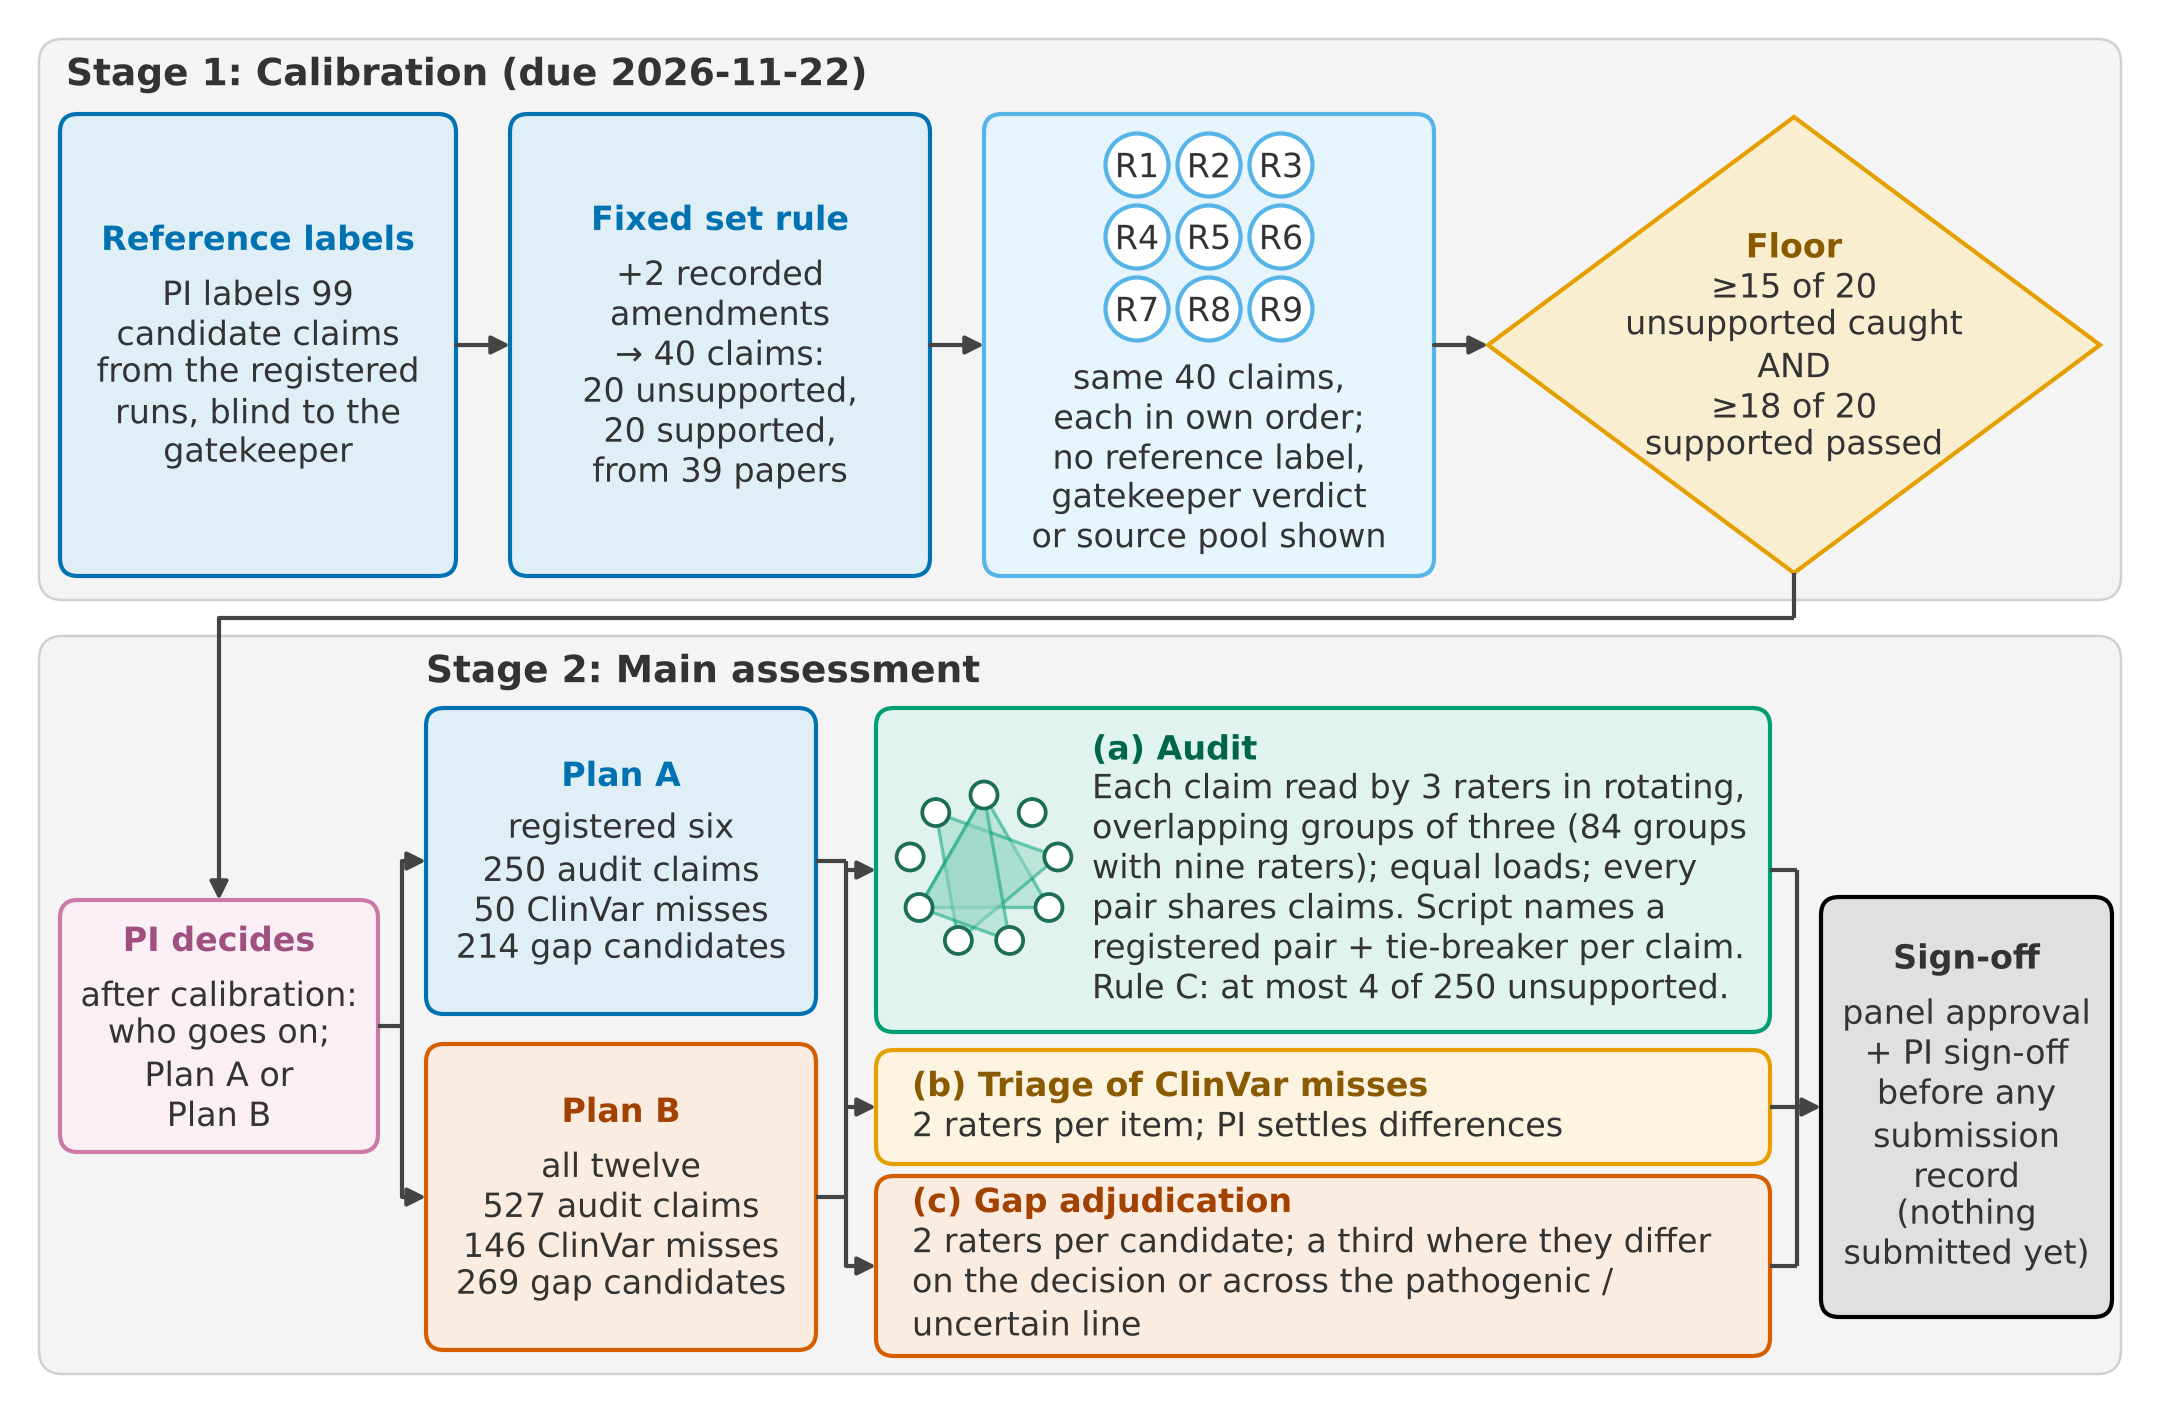
\includegraphics[width=0.68\linewidth]{figures/fig_human_assessment.png}
\end{center}
\caption{Human assessment design (D-55; procedure only, no results). Stage~1, calibration (due 2026-11-22): the PI labelled 99 candidate claims blind to the gatekeeper; a set rule fixed before any label, with two recorded amendments, selected 40 claims (20 unsupported, 20 supported, 39 papers); nine raters rate them in their own order against a floor fixed in advance. Stage~2: the PI chooses who goes on and Plan A or B (planning figures); (a) audit claims read by 3 raters in rotating groups with a registered pair and tie-breaker per claim, rule~C unchanged; (b) ClinVar misses by 2 raters; (c) gap candidates by 2 raters, a third on disagreement. Nothing is submitted without panel approval and the PI's sign-off.}
\label{fig:human}
\end{figure}

\paragraph{Design (D-55).} The PI accepted on 2026-11-15 a design of volunteer raters in rotating groups after a calibration round with a floor, in place of two fixed raters and a tie-breaker (Figure~\ref{fig:human}); nine raters take part from 2026-11-16, two of them adjudication-panel members, and none is identified. \emph{Calibration.} The PI labelled 99 candidate claims from the registered runs (outside the O1 sample; drawn both from claims the gatekeeper removed and claims it kept), blind to the gatekeeper and the source pool: 64 supported, 29 unsupported, 5 cannot verify, 1 quote not in paper. A rule fixed before any label took the first 20 labelled unsupported and the first 20 supported in seeded order. Two amendments followed his labels and preceded any rater: one kind of claim is capped on the unsupported side (kind and cap recorded privately with a committed checksum, since naming them would hint at answers), and a repeated paper and quote is skipped; both are reported wherever calibration results are. The final 40 claims come from 39 papers; 35 are shared by all three versions of the set, and results will also be given on them. How a rating counts was fixed before any rater entered one: an unsupported claim is caught when labelled unsupported, quote not in paper or cannot verify (the strict count without cannot verify reported beside it); a supported claim is passed only when labelled supported. \emph{Main assessment.} Each audit claim is read by 3 raters dealt by a seeded script over all groups of three (84 with nine raters), with a registered pair and tie-breaker per claim and rule~C unchanged; Cohen's $\kappa$ is reported per pair on shared claims, with an all-rater agreement measure beside it. Misses are triaged by 2 raters, the PI settling differences; candidates are adjudicated by 2 raters, a third where they differ on the decision or across the pathogenic / uncertain line. Registered, extension and Majeed studies are scored separately. Calibration results pending: finished \HR{cal_raters_finished} of 9; meeting the floor \HR{cal_raters_pass}; plan \HR{plan_choice} (all calibration fields in Table~\ref{tab:pending}).

\begin{table}[h]
\caption{Plan A and Plan B: planning figures, not measurements. Planning time per item: audit 1 minute (range 0.5--2; the only measurement is the pilot, 0.37 and 0.65 minutes per rating, one rater); triage 4 minutes (2--6, assumed); adjudication 15 minutes per candidate (10--30, assumed); third readings on 40\% of candidates. Calibration takes about 2.7 hours per rater.}
\begin{center}
\scriptsize
\begin{tabular}{lll}
\toprule
 & Plan A: registered six & Plan B: all twelve \\
\midrule
Extracted values audited & 250 & 527 (250 + 250 extension + 27 Majeed) \\
ClinVar misses triaged & 50 & 146 (50 + 46 + 50) \\
Gap candidates adjudicated & 214 & 269 (214 + 43 + 12) \\
Entries covered & 514 & 942 \\
Independent readings (eight raters) & 1278 + third readings & 2411 + third readings \\
Hours per rater, eight raters (range) & 21.1 (13.7--41.9) & 28.6 (17.9--56.6) \\
Rater hours in all, eight raters (range) & 169.2 (109.5--334.8) & 228.9 (143.2--453.2) \\
Weeks at 2, 3, 5 hours per rater per week (eight) & 11, 8, 5 & 15, 10, 6 \\
Hours per rater, nine raters (range) & 19.1 (12.5--37.5) & 25.7 (16.2--50.7) \\
Hours per rater, seven / six / five raters & 23.8 / 27.3 / 32.2 & 32.3 / 37.2 / 44.2 \\
\bottomrule
\end{tabular}
\end{center}
\end{table}

The PI's reference-labelling sittings for calibration took 60 ratings in 59.6 minutes (median 51 seconds between ratings), 15 in 17.2 minutes and 24 in 16.3 minutes. Gap adjudication is about 76\% of Plan A's time. Person-hours in all barely change with the number of raters (Plan A 171.9 with nine against 169.2 with eight). With nine raters, each pair shares 20 or 21 audit claims in Plan A, against 26 to 28 with eight; the plan report is written for eight raters and is to be regenerated for the final number before any audit assignment is drawn. With a cap on hours per rater, candidates fully adjudicated in Plan A: 8~h 38 of 214; 12~h 92; 16~h 145; 20~h 198; 24~h 214; in Plan B: 8~h 0 of 269; 12~h 47; 16~h 100; 20~h 154; 24~h 207; 30~h 269. What 20 unsupported calibration claims can resolve (95\% intervals): 20 of 20 caught, 83\%--100\%; 18 of 20, 68\%--99\%; 16, 56\%--94\%; 14, 46\%--88\%; 12, 36\%--81\%; a set twice as large would give 36 of 40 an interval of 76\%--97\%. The registered adjudication window is Month~4 (2026-12-21 to 2027-01-20), across the holidays; hours per rater per week are not known. Still to fix before adjudication: who gives the third reading when a panel member is one of the two adjudicators, and what counts as the panel's approval.

\section{Budget by line}
\label{app:budget}
\begin{table}[h]
\caption{Budget (estimates from chained session cost readings at list price, including helper agents; reading of 2026-11-15 16:41 UTC). Not billing figures.}
\begin{center}
\scriptsize
\begin{tabular}{rlrrr}
\toprule
\# & Line & Requested & Spent (estimate) & Remaining \\
\midrule
1 & Extraction across six diseases, incl.\ re-runs & \$8,000 & \$1,246.47 & \$6,753.53 \\
2 & Gatekeeper verification pass & \$4,000 & \$644.61 & \$3,355.39 \\
3 & ClinVar/OMIM reconciliation + concordance harness & \$6,000 & \$124.78 & \$5,875.22 \\
4 & Claude Code: pipeline, VariantValidator, dedup tooling, adjudication interface & \$6,000 & \$15.46 & \$5,984.54 \\
5 & Ascertainment-bias arm & \$4,000 & \$55.17 & \$3,944.83 \\
6 & Claude vs open-weight head-to-head & \$2,000 & \$0.00 & \$2,000.00 \\
 & Core subtotal & \$30,000 & \$2,086.49 & \$27,913.51 \\
7 & Stretch: extend to all 12 candidate diseases & \$9,000 & \$596.93 & \$8,403.07 \\
8 & Contingency & \$6,000 & \$252.62 & \$5,747.38 \\
 & Total (includes \$327.04 not assigned to a line) & \$45,000 & \$3,263.08 & \$41,736.92 \\
\bottomrule
\end{tabular}
\end{center}
\end{table}

Readings sometimes freeze or lag, and whether the sessions ran on the funded account is open (D-15); the ledger of billing figures is empty. Not counted: OpenRouter spend for the open-weight model (billed outside the award: \$16.34--\$20.35 for the two runs, about \$0.19 for the pilot and \$0.048 for its memorization probe; the key is shared, so these are upper bounds), the Majeed search session (\$19.92), the consolidation session of 2026-11-15 (its two helpers about \$5.50 by helper tokens), and claude.ai chats. The earlier total of \$1,861.06 (reading of 2026-10-24) is superseded. Unit costs: extraction about \$2 per paper by session readings (\$1.08 and \$1.19 median per paper by helper tokens on HA20 and SSADH); gatekeeper about \$0.0044 per judged claim; the six registered runs \$603 for extraction plus gatekeeper over 350 documents (\$1.72 per paper; \$1.35--2.38 by disease); HPO binding helpers \$72 against a \$28 estimate. Per-run spend: registered gap dossiers \$64.10 and Claude memorization probe \$5.34 by helper tokens; gatekeeper on the open-weight runs \$136.46; extension five \$596.93 (ceiling \$1,500); Majeed run about \$92 by helper tokens (ceiling \$120) plus about \$20 for its search screening; pilot \$673.89 against its \$1,000 ceiling. If the first deposit landed on 2026-09-21, it expires 2027-03-21; unused credits are reported, not spent for the sake of it.

\section{Memorization probe, open-weight comparison and GPSEA}
\label{app:secondary}
\begin{table}[h]
\caption{Memorization probe (exploratory; 180 papers, 30 per disease, stratified against Claude's June 2026 cutoff). One item (Tangier 33346003) excluded because its opening was publisher boilerplate. Phenotype terms: given, mapped, hits. The open-weight checkpoint's cutoff is unknown, so its strata carry no meaning.}
\begin{center}
\scriptsize
\resizebox{\linewidth}{!}{%
\begin{tabular}{lrlllllrrr}
\toprule
Stratum & Papers & Model & Closed book: specific / guess / none & Variant hit papers & Variants (hits) & Phenotype terms & ROUGE-L F1 & 5-gram share & Longest run \\
\midrule
after cutoff & 10 & Claude & 0 / 6 / 4 & 0 & 0 (0) & 24, 20, 12 & 0.158 & 0.0000 & 4 \\
after cutoff & 10 & DeepSeek & 0 / 3 / 7 & 0 & 0 (0) & 9, 1, 1 & 0.137 & 0.0000 & 4 \\
recent & 51 & Claude & 0 / 44 / 7 & 2 & 9 (2) & 163, 132, 68 & 0.190 & 0.0042 & 7 \\
recent & 51 & DeepSeek & 0 / 11 / 40 & 1 & 4 (1) & 26, 2, 1 & 0.154 & 0.0017 & 6 \\
older & 119 & Claude & 4 / 95 / 20 & 2 & 3 (2) & 306, 248, 153 & 0.190 & 0.0061 & 11 \\
older & 119 & DeepSeek & 0 / 27 / 92 & 2 & 9 (2) & 68, 31, 23 & 0.148 & 0.0021 & 7 \\
\bottomrule
\end{tabular}}
\end{center}
\end{table}

\begin{table}[h]
\caption{Claude against DeepSeek-V4.1-Flash (HA20 and SSADH, run 2026-10-21; values Claude / open-weight). Claude's cost is an estimate from helper tokens; the open-weight cost is what the host reported for final attempts.}
\begin{center}
\scriptsize
\resizebox{\linewidth}{!}{%
\begin{tabular}{lll}
\toprule
Measure & HA20 & SSADH \\
\midrule
Papers & 85 & 40 \\
Values asserted & 67,863 / 55,317 & 31,370 / 33,521 \\
Span-not-found rate & 0.00\% / 3.86\% & 0.00\% / 2.98\% \\
Values with no quote & 0 / 2,003 & 0 / 991 \\
Model claims judged by gatekeeper v4 & 23,129 / 18,084 & 9,759 / 10,372 \\
Supported / partially / unsupported / span not found & 22,683 / 400 / 46 / 0 vs 15,250 / 1,240 / 1,563 / 31 & 9,480 / 242 / 37 / 0 vs 9,020 / 715 / 637 / 0 \\
Unsupported rate (exact 95\% CI) & 0.20\% (0.15--0.27) / 8.64\% (8.24--9.06) & 0.38\% (0.27--0.52) / 6.14\% (5.69--6.62) \\
Anything but supported & 1.93\% (1.75--2.11) / 15.67\% (15.14--16.21) & 2.86\% (2.54--3.21) / 13.04\% (12.39--13.70) \\
Claims with an empty quote (judged unsupported) & 0 / 1,503 (1,185) & 0 / 591 (438) \\
Unsupported rate, claims with a quote & 0.20\% (0.15--0.27) / 2.28\% (2.06--2.52) & 0.38\% (0.27--0.52) / 2.03\% (1.76--2.33) \\
Papers with an unsupported claim & 15 / 71 & 7 / 37 \\
HGVS recall, tiers 1+2 & 26.9\% (21/78; 18.3--37.7) / 19.2\% (15/78; 12.0--29.3) & 14.6\% (23/158; 9.9--20.9) / 15.2\% (24/158; 10.4--21.6) \\
Variant keys shared/union & 261/294 (88.8\%) & 157/166 (94.6\%) \\
Checklist agreement (shared cells) & 95.9\% of 10,720 & 97.6\% of 6,716 \\
Feature rows & 5,079 / 2,753 & 1,683 / 1,439 \\
Cost per paper, median & \$1.08 / \$0.07 & \$1.19 / \$0.07 \\
Wall-clock per paper, median (min) & 2.9 / 20.9 & 2.9 / 19.2 \\
Cost, all papers & \$101.42 / \$10.25 & \$52.79 / \$5.54 \\
\bottomrule
\end{tabular}}
\end{center}
\end{table}

\paragraph{Open-weight notes.} Tier-1 overlap: HA20 37.9\% (39/103) / 41.1\% (37/90; 31.5--51.4), SSADH 87.2\% (68/78) for both; classification agreement HA20 82.8\% (24/29) / 90.0\% (18/20; 69.9--97.2), SSADH 91.8\% (45/49) / 88.5\% (46/52; 77.0--94.6). Claude-only target-gene variants 28 and open-weight-only 5 in HA20; 4 and 5 in SSADH. Counted with failed attempts, the open-weight runs cost \$16.34 to \$20.35 for 125 papers against Claude's \$154.21 estimate. Helpers did not all treat empty quotes the same way (236 HA20 and 144 SSADH empty-quote claims were judged supported against the row's quote), so the open-weight unsupported rate is, if anything, a little low. Scaffold differences: file tools only (no shell); no repair passes for empty quotes; three harness fixes during the run (retries after dropped connections, a JSON parse check on writes, a resume request never needed), approved by the PI on 2026-10-21; 13 HA20 and 1 SSADH paper were re-run from a clean start. Commonest open-weight failures: a proband flag of false with no quote; checklist statuses with no quote; a gene symbol quoted from a background sentence; an age at examination given as onset; parents' variant fields quoted from the proband's sentence; hedged findings recorded as observed.

\begin{table}[h]
\caption{Exploratory genotype--phenotype maps (GPSEA; Fisher exact tests, Benjamini--Hochberg at 0.05; individuals with a GRCh38-placed variant and at least one phenotype; zygosity for untyped calls is an analysis assumption only). The Danon truncating-vs-missense signal rests on 6--8 missense carriers and is a lead only.}
\begin{center}
\scriptsize
\begin{tabular}{lp{3.6cm}rrp{4.6cm}}
\toprule
Disease & Comparison & Individuals & Terms & Significant (BH 0.05) \\
\midrule
HA20 & truncating vs missense & 217 & 11 & 0 \\
SSADH & biallelic truncating/truncating vs truncating/other vs other/other & 77 & 9 & 0 \\
Tangier & biallelic, as above & 16 & 0 & 0 \\
LAD-I & biallelic, as above & 38 & 3 & 0 \\
AxD & hotspot R79/R88/R239 vs other missense & 83 & 14 & 0 \\
Danon & truncating vs missense & 130 & 9 & 2: arrhythmia (57/59 vs 4/7; $p_{BH}$ 0.035); ventricular arrhythmia (45/47 vs 3/6; $p_{BH}$ 0.035) \\
Danon & sex (males hemizygous, females heterozygous) & 130 & 10 & 3: proximal muscle weakness (female 1/28, male 11/25; $p_{BH}$ 0.005); left ventricular hypertrophy (25/33 vs 41/41; $p_{BH}$ 0.005); hypertrophic cardiomyopathy (19/24 vs 34/34; $p_{BH}$ 0.031) \\
\bottomrule
\end{tabular}
\end{center}
\end{table}

\paragraph{Bias-arm tags (D-48).} Tags cover 1,772 phenopackets (SSADH 464, HA20 781, Danon 527). Registered SSADH: of 311 records with a disease term, 115 are probable members of the comparator registry, 108 possible, 63 with no link. Registered HA20: 9 probable, 87 possible. Danon: nobody tagged as in the cohort. AxD is left untagged on purpose (its open comparator is UK Biobank carriers \citep{gagliardi2024_axd_ukb}). Comparators: AxD UK Biobank genotype-first cohort; Danon a prospective cohort (PMID 41121270); HA20 a multicentre preprint; SSADH a natural-history registry (PMID 30656189) \citep{dibacco2019_ssadh_natural_history}.

\section{Pilot gates and corrected application figures}
\label{app:pilot}
\begin{table}[h]
\caption{Development pilot on HA20 (2026-10-18 to 2026-10-20, before the freeze). These are development results, not general findings; the pilot's records are not used in any result table.}
\begin{center}
\scriptsize
\begin{tabular}{lp{3.5cm}p{5.0cm}}
\toprule
Gate & Threshold & Result \\
\midrule
Q1 open-access corpus & $\geq$70\% with full text & 53.1\% (85 of 160): not met \\
Q2 verbatim provenance & every value has PMID + span & 64,999 values, 100\% verbatim: met \\
Q3 valid phenopackets, normalized HGVS & 100\% valid; $\geq$95\% cDNA normalized or flagged & 749 of 749; 97.8\%: met \\
Q4 unsupported values & span match $\geq$98\%; human $\leq$4\% (n = 50) & 100\%; 6.0\% and 6.3\%: not met \\
Q5 deduplication & 0 false merges in the hand check & policy v3: 6 of 93: not met; v4: 0 of 50 (not independent) \\
Q6 concordance harness & table with CIs vs dated snapshots & met (ClinVar, HPO) \\
Q7 completeness & restricted recall $\geq$80\% & 9 of 9: met \\
Q8 cost & six-disease projection $\leq$\$8,000 & \$1,676--4,189: met \\
\bottomrule
\end{tabular}
\end{center}
\end{table}

\paragraph{Pilot audits.} First audit (instructions v3, gatekeeper v1): 3 of 50 unsupported, 6.0\% (1.3\%--16.5\%), 6 of 50 not fully supported; error class: variant fields taken from a group statement or a literature-summary column, answered by D-29. Re-audit (instructions v5, gatekeeper v3, 20 papers): 3 of 48, 6.3\% (1.3\%--17.2\%), 4 of 48 not fully supported; error class: ages read by position from a stacked multi-patient cell, which the rater could not verify, answered by D-31; without the 3 unverifiable claims, 0 of 45 (0.0\%--7.9\%). Variant fields were clean after D-29 (0 of 20 unsupported in the re-audit, against 3 of 20 before). Merge policy v3 made 93 merges; a hand check found 84 true, 6 false, 3 unclear. Measured rating time: 87 ratings in 56.7 minutes and 50 in 18.3 minutes.

\begin{table}[h]
\caption{Figures from the grant application and their corrected statements \citep{koseki2021_tangier_review,genereviews_tangier,sugie2024_danon_history,larsen2026_hpo_mcp,rao2026_reference_hallucination,jackson2025_aa_omniscience}.}
\begin{center}
\scriptsize
\begin{tabular}{p{4.3cm}p{8.6cm}}
\toprule
Application claim & Corrected statement \\
\midrule
Tangier ``$\sim$200 patients'' & Sources say fewer than 100 (GeneReviews) to about 144 (a 2021 review); use ``$\sim$100--150'' (D-14) \\
Danon ``$>$100 families'' & About 100 families; $\geq$146 molecularly confirmed patients (D-14) \\
``408 phenopacket-store cohorts'' & No published source; 731 gene folders at commit \texttt{85ffd78}, 2026-10-07 (D-14) \\
LAD-I ``genotypes for 184 patients published but never structured'' & Probably the patients \emph{without} a reported genotype (323 cases to 2017, genotype for 139), which extraction cannot recover (D-14) \\
AxD ``72 ClinVar P/LP entries; $\sim$12 OMIM allelic variants'' & 76 P/LP (release 2026-10-12, read 2026-10-19); 13 OMIM allelic variants (gene entry frozen 2026-10-28) \\
``97.6\% precision on HPO extraction (Sonnet 4.5)'' & A preprint: 4 synthetic clinical notes run $\geq$50 times, tool-augmented condition (80.7\% without tools), recall 65.3\%, not top on precision or F1; not case reports \\
``DRBench'' fabricated-citation rates 3.0\% / 3.2\% & Hallucinated-URL rates for two search-augmented Claude 3.x models (n = 641 and 1,735 URLs) on DeepResearch Bench; not fabricated citations in general \\
AA-Omniscience comparison & Each pair is real but from different model generations; compare models from one snapshot with its date \\
``ClinVar literature-only submissions'' & Submissions will use the \emph{curation} collection method (D-13) \\
\bottomrule
\end{tabular}
\end{center}
\end{table}
%%%%%%%%% Appendix %%%%%%%%%

\end{document}
